% Options for packages loaded elsewhere
\PassOptionsToPackage{unicode}{hyperref}
\PassOptionsToPackage{hyphens}{url}
\PassOptionsToPackage{dvipsnames,svgnames,x11names}{xcolor}
%
\documentclass[
]{article}

\usepackage{amsmath,amssymb}
\usepackage{lmodern}
\usepackage{setspace}
\usepackage{iftex}
\ifPDFTeX
  \usepackage[T1]{fontenc}
  \usepackage[utf8]{inputenc}
  \usepackage{textcomp} % provide euro and other symbols
\else % if luatex or xetex
  \usepackage{unicode-math}
  \defaultfontfeatures{Scale=MatchLowercase}
  \defaultfontfeatures[\rmfamily]{Ligatures=TeX,Scale=1}
\fi
% Use upquote if available, for straight quotes in verbatim environments
\IfFileExists{upquote.sty}{\usepackage{upquote}}{}
\IfFileExists{microtype.sty}{% use microtype if available
  \usepackage[]{microtype}
  \UseMicrotypeSet[protrusion]{basicmath} % disable protrusion for tt fonts
}{}
\makeatletter
\@ifundefined{KOMAClassName}{% if non-KOMA class
  \IfFileExists{parskip.sty}{%
    \usepackage{parskip}
  }{% else
    \setlength{\parindent}{0pt}
    \setlength{\parskip}{6pt plus 2pt minus 1pt}}
}{% if KOMA class
  \KOMAoptions{parskip=half}}
\makeatother
\usepackage{xcolor}
\setlength{\emergencystretch}{3em} % prevent overfull lines
\setcounter{secnumdepth}{5}
% Make \paragraph and \subparagraph free-standing
\ifx\paragraph\undefined\else
  \let\oldparagraph\paragraph
  \renewcommand{\paragraph}[1]{\oldparagraph{#1}\mbox{}}
\fi
\ifx\subparagraph\undefined\else
  \let\oldsubparagraph\subparagraph
  \renewcommand{\subparagraph}[1]{\oldsubparagraph{#1}\mbox{}}
\fi


\providecommand{\tightlist}{%
  \setlength{\itemsep}{0pt}\setlength{\parskip}{0pt}}\usepackage{longtable,booktabs,array}
\usepackage{calc} % for calculating minipage widths
% Correct order of tables after \paragraph or \subparagraph
\usepackage{etoolbox}
\makeatletter
\patchcmd\longtable{\par}{\if@noskipsec\mbox{}\fi\par}{}{}
\makeatother
% Allow footnotes in longtable head/foot
\IfFileExists{footnotehyper.sty}{\usepackage{footnotehyper}}{\usepackage{footnote}}
\makesavenoteenv{longtable}
\usepackage{graphicx}
\makeatletter
\def\maxwidth{\ifdim\Gin@nat@width>\linewidth\linewidth\else\Gin@nat@width\fi}
\def\maxheight{\ifdim\Gin@nat@height>\textheight\textheight\else\Gin@nat@height\fi}
\makeatother
% Scale images if necessary, so that they will not overflow the page
% margins by default, and it is still possible to overwrite the defaults
% using explicit options in \includegraphics[width, height, ...]{}
\setkeys{Gin}{width=\maxwidth,height=\maxheight,keepaspectratio}
% Set default figure placement to htbp
\makeatletter
\def\fps@figure{htbp}
\makeatother
\newlength{\cslhangindent}
\setlength{\cslhangindent}{1.5em}
\newlength{\csllabelwidth}
\setlength{\csllabelwidth}{3em}
\newlength{\cslentryspacingunit} % times entry-spacing
\setlength{\cslentryspacingunit}{\parskip}
\newenvironment{CSLReferences}[2] % #1 hanging-ident, #2 entry spacing
 {% don't indent paragraphs
  \setlength{\parindent}{0pt}
  % turn on hanging indent if param 1 is 1
  \ifodd #1
  \let\oldpar\par
  \def\par{\hangindent=\cslhangindent\oldpar}
  \fi
  % set entry spacing
  \setlength{\parskip}{#2\cslentryspacingunit}
 }%
 {}
\usepackage{calc}
\newcommand{\CSLBlock}[1]{#1\hfill\break}
\newcommand{\CSLLeftMargin}[1]{\parbox[t]{\csllabelwidth}{#1}}
\newcommand{\CSLRightInline}[1]{\parbox[t]{\linewidth - \csllabelwidth}{#1}\break}
\newcommand{\CSLIndent}[1]{\hspace{\cslhangindent}#1}

\usepackage{fancyhdr}
\pagestyle{fancy}
\fancyhead[L]{Candidate 7}
\fancyhead[C]{Term Paper ECS530}
\fancyhead[R]{02-06 jan 2023}
\fancyfoot[CO,CE]{\thepage}
\usepackage{sectsty}
\definecolor{overskrift}{RGB}{0,175,186}
\allsectionsfont{\color{overskrift}}
\usepackage[labelfont=bf]{caption}
\usepackage{float}
\floatplacement{table}{H}
\makeatletter
\makeatother
\makeatletter
\makeatother
\makeatletter
\@ifpackageloaded{caption}{}{\usepackage{caption}}
\AtBeginDocument{%
\ifdefined\contentsname
  \renewcommand*\contentsname{Table of contents}
\else
  \newcommand\contentsname{Table of contents}
\fi
\ifdefined\listfigurename
  \renewcommand*\listfigurename{List of Figures}
\else
  \newcommand\listfigurename{List of Figures}
\fi
\ifdefined\listtablename
  \renewcommand*\listtablename{List of Tables}
\else
  \newcommand\listtablename{List of Tables}
\fi
\ifdefined\figurename
  \renewcommand*\figurename{Figur}
\else
  \newcommand\figurename{Figur}
\fi
\ifdefined\tablename
  \renewcommand*\tablename{Tabell}
\else
  \newcommand\tablename{Tabell}
\fi
}
\@ifpackageloaded{float}{}{\usepackage{float}}
\floatstyle{ruled}
\@ifundefined{c@chapter}{\newfloat{codelisting}{h}{lop}}{\newfloat{codelisting}{h}{lop}[chapter]}
\floatname{codelisting}{Listing}
\newcommand*\listoflistings{\listof{codelisting}{List of Listings}}
\makeatother
\makeatletter
\@ifpackageloaded{caption}{}{\usepackage{caption}}
\@ifpackageloaded{subcaption}{}{\usepackage{subcaption}}
\makeatother
\makeatletter
\@ifpackageloaded{tcolorbox}{}{\usepackage[many]{tcolorbox}}
\makeatother
\makeatletter
\@ifundefined{shadecolor}{\definecolor{shadecolor}{rgb}{.97, .97, .97}}
\makeatother
\makeatletter
\makeatother
\ifLuaTeX
\usepackage[bidi=basic]{babel}
\else
\usepackage[bidi=default]{babel}
\fi
\babelprovide[main,import]{norsk}
% get rid of language-specific shorthands (see #6817):
\let\LanguageShortHands\languageshorthands
\def\languageshorthands#1{}
\ifLuaTeX
  \usepackage{selnolig}  % disable illegal ligatures
\fi
\IfFileExists{bookmark.sty}{\usepackage{bookmark}}{\usepackage{hyperref}}
\IfFileExists{xurl.sty}{\usepackage{xurl}}{} % add URL line breaks if available
\urlstyle{same} % disable monospaced font for URLs
\hypersetup{
  pdftitle={Masteroppgave},
  pdfauthor={Morten Knutsen og Sindre M. Espedal},
  pdflang={nb-NO},
  colorlinks=true,
  linkcolor={blue},
  filecolor={Maroon},
  citecolor={teal},
  urlcolor={teal},
  pdfcreator={LaTeX via pandoc}}

\title{Masteroppgave}
\author{Morten Knutsen og Sindre M. Espedal}
\date{}

\begin{document}
\maketitle
\ifdefined\Shaded\renewenvironment{Shaded}{\begin{tcolorbox}[interior hidden, boxrule=0pt, breakable, sharp corners, borderline west={3pt}{0pt}{shadecolor}, enhanced, frame hidden]}{\end{tcolorbox}}\fi

\setstretch{1.5}
\hypertarget{introduksjon-beyonder-og-haugaland-nuxe6ringspark}{%
\section{Introduksjon Beyonder og Haugaland
næringspark}\label{introduksjon-beyonder-og-haugaland-nuxe6ringspark}}

Beyonder er en batteribedrift som har planer om å etablere en
gigafabrikk (Whiteaker, 2022) på Haugaland næringspark i Gismarvik. Den
kommersielle distribusjonen fra fabrikken er planlagt fra 2026
(Beyonder, 2022). I første omgang ser Beyonder for seg å ansette mellom
800-1000 arbeidstakere for å drifte de fem første produksjonshallene. De
ser for seg i senere tid å etablere fem ekstra haller og med det sitte
med 10 haller og da trenger cirka 2000 ansatte hvorav 70-75\% vil være
fagarbeidere, 25-30\% vil være ingeniører og i tillegg en administrasjon
bestående av ledelse, økonomi, HR, HMS, supply chain osv. De ser for seg
at de trenger cirka 50 ansatte i administrasjonen per 1000 ansatte.
Administrasjon kan ende opp med 100 ansatte.

Beyonder var første produsent av batteri-celler i Norge og ble etablert
i slutten av første kvartal i 2016. Beyonder har stadig utviklet seg og
har i dag 59 ansatte (Proff, 2023). Beyonder produserer såkalte
«høyeffektsbatterier», som er batterier med mye kraft. Batteriene er en
hybrid mellom en kondensator og et lithiumion batteri, dette er med på å
løse utfordringer som ikke er adressert i dagens batterier. Batteriene
er også øko-vennlige, og produksjonen består av bruk av fornybar energi
og sagspon (Beyonder, 2023b).

Beyonder planlegger å etablere en gigafabrikk på Haugaland Næringspark,
lokalisert i Gismarvik. Valg av destinasjon er en nøye vurdering av
lokalsamfunn, naturomgivelser, tilgang på personell og ren kraft
(Beyonder, 2023a). Gigafabrikken er planlagt å være ferdig innen 2026.

Haugaland næringspark er Norges største regulerte næringspark og gir
bedrifter gode muligheter til å utforme tomt etter ønske(Haugaland
næringspark, 2023). Området er spesielt lagt til rette for areal- og
energikrevende industri, noe Beyonder er. Det er også god tilgang til
kraft i form av el-kraft, naturgasser og fornybar kraft. Næringsparken
har også lett tilkomst med bilvei og sjøveien (Haugaland næringspark,
2023). I tillegg er det ikke langt fra Haugesund flyplass, Karmøy, noe
som gjør beliggenheten veldig tilgjengelig. Gismarvik Havn som er en del
av Haugesund næringspark har en kai på 110 meter og minste dybde på 16,5
meter, noe som betyr at tilkomst med båt ikke er noe problem og kan være
med på å øke attraktiviteten til å etablere seg her(næringspark, 2023).
Det er også et lagerareal på 80 dekar, dette gjør at bedrifter som er
etablert i næringsparken kan lagre ferdigprodukt på kaien og ligger der
klar til henting av båter. En slik næringspark passer veldig godt inn i
etableringen til Beyonder. Næringsparken vil bidra med gode forbindelser
til både vann, land og luft som gjør at produktene enkelt kan
distribueres rundt.

\hypertarget{beyonder-bare-et-luftslott}{%
\subsection{Beyonder, bare et
luftslott?}\label{beyonder-bare-et-luftslott}}

Etableringen av Beyonder på Gismarvik er fortsatt i veldig tidlig fase,
og for at det skal realiseres må det hentes inn milliarder i kapital
(Størksen, 2022b). På starten av 2023 leter Beyonder etter finansiering
til hovedkontoret og driften på Forus, og etablering på Gismarvik er
ikke i fokus (Størksen, 2023). Beyonder sin manglende langsiktige
finansiering skaper stor usikkerhet og betydelig tvil om selskapets evne
til fortsatt drift (Størksen, 2022a). Dette har skapt debatt i
lokalsamfunnet, og det har vokst frem skepsis om det er et luftslott som
planlegges på Haugaland næringspark (Kristensen, 2022).

En annen mulig skepsis som kan være i samfunnet er uroen for
``backwash-effekter'' (Capello, 2015), som handler om at konkurransen i
regionen øker, og presser opp lønninger, ved en etablering av
batterifabrikken. Denne økte konkurransen kan føre til at andre
bedrifter blir til slutt utkonkurrert. Backwash-effekter vil bli
presentert og diskutert grundigere i (\textbf{chp-FINN?}) DETTE

\hypertarget{tilrettelegging-av-etablering-puxe5-gismarvik}{%
\subsection{Tilrettelegging av etablering på
Gismarvik}\label{tilrettelegging-av-etablering-puxe5-gismarvik}}

I oppgaven har vi valgt å se på Beyonder da det er den bedriften som er
aktuell med etablering i Gismarvik. Med den tilrettelagte
infrastrukturen og en strategisk god beliggenhet i regionen er det ikke
urimelig å forvente andre etableringer. Vår analyse av ringvirkninger er
relevant for etableringer generelt, og er ikke knyttet spesifikt til
batteriproduksjon.

Viktige forhold i en ringvirkningsanalyse er om det oppstår generative
eller distributive virkninger. En distributiv virkning får vi når et
område har en positiv utvikling og motsvares av en tilsvarende negativ
utvikling i et annet område. Et godt eksempel på en slik virkning er
flyttestrømmer. Flyttestrømmer kan også være en naturlig del av en
generativ prosess, med flytting mellom ulike geografiske områder.
Generativ virkning kan for eksempel være utvikling av veinett som vil
gjøre arbeidsmarkedet mer effektivt, hvis det oppstår en generativ
effekt vil dette gi en forbedring i geografien som helhet (Bråthen et
al., 2003). Over tid har det blitt investert i forbedring av veinett på
Haugalandet gjennom Haugalandspakken. Det er fine veier inn til
Haugaland næringspark, noe som gjør det lett tilgjengelig. Dette er med
på å skape kortere reisetid for varer som blir produsert, noe igjen som
gjør varene mer attraktive. Nå som arbeidet av Rogfast er i gang
(Statens vegvesen, 2023) vil ferdigstillingen av denne være med på å øke
tilgjengeligheten mellom Haugalandet og Stavanger-regionen og det kan
skape enda større generative effekter for regionen. Generative
virkninger kan for eksempel forklares med klyngegevinster, dette oppstår
med en sterkere konsentrasjon av næringsvirksomhet i en geografi. Dette
blir forklart gjennom en prosess med ``learning, sharing and matching''
(Duranton og Puga, 2003). Dette vil vi utdype mer i neste kapittel.

\hypertarget{en-deskriptiv-gjennomgang-av-nuxe6ringsstruktur-og-arbeidsmarked-puxe5-haugalandet}{%
\section{En deskriptiv gjennomgang av næringsstruktur og arbeidsmarked
på
Haugalandet}\label{en-deskriptiv-gjennomgang-av-nuxe6ringsstruktur-og-arbeidsmarked-puxe5-haugalandet}}

I dette kapittelet ønsker vi å få et grunnlag for å vurdere hvordan en
batteribedrift kan tenkes å tilpasse seg næringslivet på Haugalandet.
Det kan tenkes at Beyonder vil inngå i en klynge av industribedrifter
som kan oppnå fordeler knyttet til ``sharing, matching and learning''
(Duranton og Puga, 2003). ``Sharing'' handler om hvordan bedriftene i
denne regionen deler på ressursene og kunnskapen som er tilgjengelig i
regionen. Eksempler på sharing oppstår gjennom nettverk, samarbeid og
kunnskapsbaserte tjenester. Dette bidrar til å skape et miljø med høyere
innovasjon og dynamikk. Dette er med på å skape rom for effektivisering
representert ved at det etableres bedrifter som bidrar med
fellestjenester til andre bedrifter, som slipper å etablere egne
avdelinger for slike funksjoner, knyttet til lovgiving, regnskap,
ingeniørtjenester o.l.

``Matching'' refererer til at arbeidstakere og bedrifter i urbane
områder finner hverandre og samhandler på en mer effektiv måte, for
eksempel gjennom bedriftsnettverk og rekrutteringsprosesser. Dette kan
bidra til å redusere informasjonsasymmetrier og transaksjonskostnader,
og dermed øke produktiviteten og veksten. Glaeser (2010) mener at
``matching'' er en av de viktigste faktorene som bidrar til
produktivitetsøkning i urbane områder, og at det kan føre til at byene
tiltrekker seg stadig mer kvalifisert arbeidskraft og innovative
bedrifter. ``Matching'' sier også noe om hvordan turnoveren er i
bransjen. Den tar også frem at det er lik type arbeidskraft som trengs
hos de forskjellige bedriftene og med det gjør det lettere å få
rekruttere arbeidskraft fra for eksempel andre bedrifter. Fordeler med
dette er at du slipper opplæringskostnader fordi de kan store deler av
jobben de skal inn i, fra før.

``Learning'' refererer til at arbeidstakere og bedrifter i urbane
områder får tilgang til og tilegner seg ny kunnskap og ferdigheter
gjennom ulike former for opplæring, utdanning og erfaring. Dette kan øke
produktiviteten og effektiviteten i bedriftene og dermed bidra til
økonomisk vekst (Duranton og Puga, 2004). Glaeser (2010) understreker
også viktigheten av læring i urbane områder og hvordan det kan føre til
innovasjon og økt produktivitet. Han argumenterer for at byer gir
mulighet for folk å lære av hverandre, og at dette kan føre til at ideer
og innovasjoner spres raskere og bredere. På en annen side kan det også
være utfordringer knyttet til læring i urbane områder. Duranton og Puga
(2004) argumenterer for at det kan være begrensninger på læring på grunn
av ujevnhet i ressurstilgang og ulike erfaringer i forskjellige
bedrifter. Dette kan gjøre det vanskelig for mindre bedrifter og
nykommere å lære og tilpasse seg like mye som større, etablerte
bedrifter.

Slike klyngefordeler gir rom for effektivitetsgevinster for en region,
samlet sett, men i en slik prosess kan det også være at enkelte deler av
regionen, for eksempel i relativt perifer beliggenhet til klyngen, kan
tape både befolkning og arbeidsplasser. Sauda er et eksempel på et slikt
område i regionen

Klyngeteori er en økonomisk teori som hevder at bedrifter som er
lokalisert i nærheten av hverandre, eller i en klynge, kan ha økonomiske
fordeler som ikke er tilgjengelige for bedrifter som er lokalisert
utenfor klyngen. Denne teorien ble først utviklet av den britiske
økonomen Alfred Marshall i hans bok ``Principles of Economics'' fra
1920.

Marshall (2009) mente at nærhet mellom bedrifter i en klynge kan føre
til økt produktivitet og innovasjon, fordi bedriftene kan dra nytte av
eksternaliteter som kunnskapsoverføring og felles tilgang til
infrastruktur og arbeidskraft. Marshall argumenterte også for at klynger
kan gi bedrifter en økt konkurranseevne ved å tillate dem å dele på
kostnader og risiko.

Senere har forskere videreutviklet Marshalls teori og studert klynger i
ulike sammenhenger. Hoover (1948) undersøkte geografisk lokalisering av
bedrifter og økonomisk aktivitet og argumenterte for at nærhet mellom
bedrifter i en klynge kan føre til reduserte transaksjonskostnader og
økt innovasjon.

Cooke (2001) har også studert klynger og pekt på at klynger kan ha både
positive og negative konsekvenser for økonomisk utvikling. Han
argumenterer for at klynger kan føre til økt innovasjon og
produktivitet, men også til økt økonomisk ulikhet mellom regioner.

Paci og Usai (1999) studerte eksternaliteter og kunnskapsoverføringer i
klynger og fant at kunnskapsspredning mellom bedrifter i en klynge kan
føre til økt innovasjon og produktivitet, spesielt for små og
mellomstore bedrifter. De påpeker imidlertid også at
kunnskapsoverføringen ikke nødvendigvis skjer jevnt mellom alle
bedrifter i klyngen, og at større bedrifter ofte kan dra større nytte av
klyngens ressurser og nettverk.

Henderson (1997) har studert eksternaliteter og industriell utvikling og
funnet at nærhet mellom bedrifter kan føre til økt innovasjon og
produktivitet, men også til økte kostnader på grunn av miljøproblemer og
konkurranse om ressurser.

Glaeser et al. (1992) har studert vekst i byer og funnet at nærhet
mellom bedrifter kan føre til økt innovasjon og produktivitet, men også
til økt konkurranse og konflikt mellom bedrifter.

Samlet sett kan klyngeteori være et nyttig rammeverk for å forstå
økonomisk vekst og utvikling i regioner og byer. Det gir innsikt i
hvordan lokale økonomiske faktorer kan samhandle og skape fordeler og
ulemper for bedrifter i området. Klyngeteorien understreker også
viktigheten av eksterne effekter og kunnskapsspredning, noe som kan
bidra til å stimulere innovasjon og økonomisk vekst i klyngen.

Selv om klyngeteorien har blitt anerkjent som en verdifull tilnærming
til å forstå økonomisk utvikling, har den også møtt kritikk for en rekke
begrensninger og utfordringer. Cooke (2001) argumenterer for at
klyngeteorien kan føre til en overdreven vektlegging av økonomisk
konkurranse innenfor en klynge, og at den ikke tar hensyn til
ikke-markedsmessige faktorer som politikk og kultur. Maskell og Malmberg
(1999) har også pekt på utfordringene med å definere og måle klynger og
deres effekter nøyaktig. Storper (1997) kritiserte klyngeteorien for å
være for lite opptatt av sammenhengen mellom lokale og globale
økonomier. Bathelt et al. (2004) hevder at klyngeteorien overser
viktigheten av kunnskap som flyter gjennom globale nettverk, og at det
er behov for en mer dynamisk og kompleks tilnærming til å forstå
økonomisk utvikling.

Til tross for disse begrensningene, fortsetter klyngeteorien å være et
viktig perspektiv innen økonomisk geografi og regional utvikling.
Forskning innenfor dette feltet vil sannsynligvis fortsette å gi innsikt
i hvordan klynger fungerer, og hvordan de kan bidra til å fremme
økonomisk vekst og utvikling på lokalt og regionalt nivå.

Vi kan også se på ``learning regions'' i Capello (2015). Her får vi et
innblikk i hva som blir sitt på viktige egenskaper i en region for at
bedrifter skal lykkes. Den viktigste ressursen er kunnskap. For å få
kunnskap kreves det læring og læring springer ut av samarbeid og
interaksjon mellom bedriftene, kunder og bedrifter og interaksjon innad
i bedriften. Med å etablere seg i en industriklynge som Haugalandet er,
er det mange fordeler Beyonder kan dra med seg. Et eksempel er transport
av varer på sjø og land, lære av andre store bedrifter hva som er mest
hensiktsmessig. Men er det riktig og nok arbeidskraft til å drifte
fabrikken? Er det muligheter å få hente industriarbeidere fra andre
relevante jobber? Dette skal vi se på videre i oppgaven.

Tradisjonelt sett består regionen Haugalandet av kommunene Haugesund,
Bokn, Tysvær, Karmøy, Utsira, Vindafjord (Thorsnæs, 2021). Vi har også
valgt å se på Etne og Sveio kommune på grunn av deres nærhet til
regionen i geografien. Bømlo og Stord kommune ligger nesten like tett på
Gismarvik som Etne, men etter en vurdering ut fra pendledataene så
utelates Stord og Bømlo. Oppgavens begrensninger i form av tid er også
en faktor for denne avgjørelsen, selv om det kan diskuteres om dette er
en god beslutning. Sauda kommune ligger enda lengre fra Gismarvik, men
kan tenkes å tjene som et eksempel på en lokal kommune som er mer
perifert knyttet til anlegget på Gismarvik. Vi ender derfor opp med å se
på kommunene på Haugalandet, i tillegg til Etne-, Sveio- og Sauda
kommune.

\hypertarget{den-geografiske-fordelingen-av-arbeidsplasser-puxe5-haugalandet}{%
\subsection{Den geografiske fordelingen av arbeidsplasser på
Haugalandet}\label{den-geografiske-fordelingen-av-arbeidsplasser-puxe5-haugalandet}}

Vi starter med en illustrasjon av en helhetlig beskrivelse knyttet til
fordelingen av arbeidsplasser mellom de lokale kommunene. Det aller
meste av regionen kan oppfattes som et felles bo- og
arbeidsmarkedsområde (BA-region), hvor mye av pendlestrømmen til
arbeidsplasser flyter inn til Haugesund. Det kommer også pendlestrømmer
fra/til kommunene Bømlo og Stord. Som nevnt foran, er likevel ikke disse
kommunene en del av dataene i presentasjonen av dette kapittelet.
Pendledataene er også sett i forhold til regionen, så pendlestrømmer som
flyter utenfor dette området er ikke med i beregningene. Dataene fra
Figur~\ref{fig-sysselsettingsfordeling} og Figur~\ref{fig-innpendling}
er hentet fra tabellene 13470 og 03321 hos SSB (se appendiks). I
Figur~\ref{fig-sysselsettingsfordeling} er dataene registrert av
sysselsatte personer etter arbeidssted. Alle næringene er summert opp
kolonnevis i pendlematrisene, og ender da opp med et estimat for antall
personer som arbeider i kommunene. Disse er da delt på alle sysselsatte
i kommunene samlet sett for regionen, slik at vi får en andelsfordeling
mellom kommunene av sysselsatte etter arbeidssted i regionen. Dataene
presentert i Figur~\ref{fig-sysselsettingsfordeling} gjelder for året
2021.

Figur~\ref{fig-sysselsettingsfordeling} viser tydelig at Haugesund
kommune har den høyeste andelen sysselsatte etter arbeidssted i
regionen. I tabell 03321 finner vi at de som har arbeidsstedsadresse i
Haugesund kommune, har 55,8\% av disse Haugesund kommune som bosted.
23,6\% av de som jobber i Haugesund har bosted i Karmøy kommune. 7,5\%
av disse har bosted i Tysvær kommune, og 4\% har bostedsadresse i Sveio
kommune. De resterende 9\% er jevnt spredt mellom kommune i regionen og
resten av landet. Karmøy kommune, som er den mest befolkede kommunen i
regionen, har den nest høyest andelen av sysselsatte etter arbeidssted
på Haugalandet. Av de som har arbeidsstedsadresse i Karmøy kommune, har
16\% av disse bosted i Haugesund kommune. 4\% har bostedsadresse i
Tysvær kommune. 73,1\% har både bosteds- og arbeidsadresse i Karmøy
kommune. De 7\% som gjenstår er spredt mellom de gjenstående kommunene i
regionen og resten av landet.

Figur~\ref{fig-innpendling} viser at Tysvær er den kommunen med høyest
andel av innpendlere i regionen. Omtrent halvparten av de som pendler
inn til Tysvær kommer fra Haugesund, med en andel på 46,7\%. Karmøy
kommune står for 33\% av innpendling til Tysvær. Vindafjord har 10,3\%
av innpendlingen til Tysvær, og Sveio står for 6,8\% av pendling inn til
kommunen.

Tysvær kommune har også en høy andel med 53,9\% av arbeidere som pendler
ut av kommunen. Av de som pendler ut av Tysvær kommune, pendler 61,2\%
av de til Haugesund kommune. Nest høyeste andelen pendler til Karmøy,
med en andel rundt 24,1\%. 11\% av arbeidstakerne i Tysvær pendler til
Vindafjord.

I midtre strøk i regionen har Vindafjord mange arbeidsplasser og mye
innpendling sett i forhold til nabokommunen Etne. Dette reflekterer
klyngen av store bedrifter i Ølensvåg, som bedriftene Ølen Betong,
Westcon, Berge sag og Omega365.

Denne skjeve fordelingen av arbeidsplasser i forhold til folketallene i
kommunen kan forklares i pendledataene. Det er høy interkommunal
interaksjon i arbeidsmarkedet i regionen. Figur~\ref{fig-innpendling}
illustrerer et bilde på hvordan pendlestrømmene flyter rundt mellom
kommunene i regionen. Haugesund og Tysvær er de kommunene som har størst
antall arbeidsplasser per innbygger.
Figur~\ref{fig-sysselsettingsfordeling} og Figur~\ref{fig-innpendling}
reflekterer også at disse kommunene er de mest sentralt beliggende i
geografien, sett i forhold til mulighetene for interaksjon med
nabokommuner.

Sauda er den kommunen i regionen med lavest andel innpendling. Sauda har
også en høy andel på 96\% av sysselsatte som bor og arbeider i samme
kommune. Dette er desidert høyest i regionen, med unntak for Utsira, som
er i en veldig spesiell lokalisering. Dette reflekterer Sauda sin
perifere beliggenhet når det gjelder tilgjengelighet til arbeidsplasser,
og til alt annet.

\begin{figure}[H]

{\centering \includegraphics{Masteroppgave_files/figure-pdf/fig-sysselsettingsfordeling-1.pdf}

}

\caption{\label{fig-sysselsettingsfordeling}Andel sysselsatte etter
arbeidssted, 2021}

\end{figure}

\begin{verbatim}
Warning: Using `size` aesthetic for lines was deprecated in ggplot2 3.4.0.
i Please use `linewidth` instead.
\end{verbatim}

\begin{figure}[H]

{\centering \includegraphics{Masteroppgave_files/figure-pdf/fig-innpendling-1.pdf}

}

\caption{\label{fig-innpendling}Innpendling, som en andel av
arbeidsplassene i kommunene, 2000 - 2020}

\end{figure}

\hypertarget{andelen-sysselsatte-i-ulike-nuxe6ringer}{%
\subsection{Andelen sysselsatte i ulike
næringer}\label{andelen-sysselsatte-i-ulike-nuxe6ringer}}

Motivasjonen for dette kapittelet er å få frem hvordan næringsstrukturen
ser ut på Haugalandet. Vi vil skape et bilde på hva Haugalandet er
spesialisert i, dette vil vi gjøre med å sette næringer opp mot
hverandre på region- og landsbase. Ved å danne et bilde av
næringsstrukturen kan vi få informasjon for å registrere eventuelle
klynger, og få grunnlag for å vurdere hvordan en ny industribedrift på
Gismarvik eventuelt kan supplere eksisterende næringsstruktur på en måte
som kan forsterke eventuelle klyngeeffekter.

Vi starter med en presentasjon av næringsfordelingen på Haugalandet
sammenlignet med næringsfordelingen ellers i landet, ved hjelp av
kakediagrammene i Figur~\ref{fig-kake-haugalandet} og
Figur~\ref{fig-kake-norge}.

I kakediagrammene vi har fremstilt under så får vi et inntrykk på
hvordan næringsinndelingen lokalt avviker fra den nasjonale inndelingen.
Her får vi frem at det største avviket fra landsgjennomsnittet gjelder
industrinæringen. På et så aggregert nivå, geografisk og næringsmessig,
er dette helt naturlig. Slike forskjeller er å forvente for typiske
basenæringer. Basenæring er en næring som eksporterer varer og tjenester
ut av regionen, mens bedrifter innenfor lokalnæringene i hovedsak
betjener befolkningen internt i regionen. Dette vil bli mer forklart i
kapittel 3 og 4 om baseteori og anvendelsen.

Videre i oppgaven vil vi se på næringer på 2-siffer nivå, der vi vil gå
mer detaljert inn å se på hvilke næringer som er tyngre vektet på
Haugalandet enn Norge. Dette er for å få en bedre innsikt i hvilken
arbeidskraft som er på Haugalandet og hvordan utviklingen har vært de
siste årene. Appendix 1 gir oversikt og forklaring på næringsfordelingen
etter ulike siffernivåer av NACE-koder. NACE er en EU-standard for
næringsgrupperinger som brukes til statiske formål. Ifølge Statistisk
sentralbyrå (2023) er NACE-hovednivå det samme som NACE-seksjon, som er
det øverste nivået i NACE-systemet. Dette nivået består av 21 seksjoner
som hver representerer en bred kategori av økonomisk aktivitet, for
eksempel ``Jordbruk, skogbruk og fiske'' eller ``Informasjon og
kommunikasjon''. Seksjonene er nummerert fra A til U.

\begin{figure}[H]

{\centering \includegraphics{Masteroppgave_files/figure-pdf/fig-kake-haugalandet-1.pdf}

}

\caption{\label{fig-kake-haugalandet}Næringsinndelingen på
NACE-nivå,hovedgrupper, Haugalandet 2021}

\end{figure}

\begin{figure}[H]

{\centering \includegraphics{Masteroppgave_files/figure-pdf/fig-kake-norge-1.pdf}

}

\caption{\label{fig-kake-norge}Næringsinndelingen på NACE-nivå,
hovedgrupper, Norge 2021}

\end{figure}

\hypertarget{lokaliseringskvotienter}{%
\subsubsection{Lokaliseringskvotienter}\label{lokaliseringskvotienter}}

Med å se på lokaliseringskvotienter (LQ) så får vi en oversikt over
hvordan næringsstrukturen til regionen er og hvilke næringer som er
base- eller lokalnæring i en region. Krugman (1991) forklarer at en
lokaliseringskvotient er et mål på den relative konsentrasjonen av en
bransje eller økonomisk aktivitet i en bestemt region, sammenlignet med
en større geografisk enhet. Dette verktøyet brukes ofte i økonomisk
geografi for å analysere regionale ulikheter i økonomisk utvikling og er
en god indikator til å få fram kjennetegn ved den lokale
næringsstrukturen. Capello (2015) forklarer videre at dersom LQ er
større enn én, betyr det at denne sektoren er overrepresentert i
regionen, og omvendt, hvis kvotienten er mindre enn én, betyr det at
sektoren er underrepresentert.@mccann viser til følgende LQ formel:

\(LQ_{ir} = \frac{\frac{E_{ir}}{E_r}}{\frac{E_{in}}{E_n}}\) .

Hvor \(E_{ir}\) er sysselsetting i sektor \(i\) for region \(r\).
\(E_r\) er samlet sysselsetting i region \(r\). Og \(E_{in}\) er da
nasjonal sysselsetting i sektor \(i\), og \(E_n\) er samlet nasjonal
sysselsetting.

I Figur~\ref{fig-loq} har vi tatt utgangspunkt i næringer som har
verdier større enn 1 på NACE-hovednivå. Videre nedover i hierarkiet har
vi delt opp næringene i underkategorier på 2-siffernivå. Slik oppnår vi
en mer detaljert forklaring på kjennetegn ved den lokale
næringsstrukturen i regionen, og vil gi bedre grunnlag for å beskrive og
forklare eventuelle klynger. Resultatene fra Figur~\ref{fig-loq} gir
grunnlaget for de utvalgte næringene i seksjonene under.

\begin{figure}[H]

{\centering \includegraphics{bilder/LQ-hierarki.png}

}

\caption{\label{fig-loq}LQ-verdier for Haugalandet, etter næring}

\end{figure}

\hypertarget{fiske-fangst-og-akvakultur-sjuxf8fart}{%
\subsubsection{Fiske, fangst og akvakultur \&
Sjøfart}\label{fiske-fangst-og-akvakultur-sjuxf8fart}}

Figur~\ref{fig-ffa} viser at Haugalandet har en høyere andel sysselsatte
i fiske, fangst og akvakultur enn det som er situasjonen for nasjonen
som helhet. Haugalandet har hatt en vekst i næringen på 34,56\% i antall
sysselsatte mellom perioden 2008-2021. Norge har hatt en vekst på
27,61\% i tilsvarende periode. I regionen står Karmøy kommune med den
høyeste andelen av sysselsatte i fiske, fangst og akvakultur med cirka
30\%.

Figur~\ref{fig-ffa} viser at andelen sysselsatte på Haugalandet er
markant større enn andelen nasjonalt i næringen sjøfart. En mulig
forklaring på denne forskjellen er regionen sin rolle i den maritime
næringen. Mange mener Haugesund er den maritime hovedstaden i Norge,
dette kan støttes opp av at Sjøfartsdirektoratet ble flyttet fra Oslo
til Haugesund i 2006 (Sjøfartsdirektoratet, 2023). Solstad shipping og
Knutsen OAS shipping er eksempler på to sentrale bedrifter som påvirker
størrelsen på sjøfartsnæringen her på Haugalandet. I 2014 oppsto
oljekrisen i Norge, i hovedsak Vest-Norge (Ntb, 2016). Det er derfor vi
ser en stor nedgang i andel ansatte på Haugalandet innen sjøfart fra
2014 til 2016. Vi ser at det er tendenser til vekst i sjøfart næringen
fra og med 2020 og videre. Dette kan ha noe med optimismen og
etableringen av havvindparker {[}FornybarNorge (2022). Til etableringen
av havvindparker så krever det sysselsatte i sjøfartsnæringen for å
gjennomføre prosjektene. Solstad offshore, Deepocean og Aker Solutions
etablerte i 2021 selskapet Offshore Renewables Alliance. Denne
etableringen er med på å gi et oppsving til sjøfartnæringen lokalt (Aker
Solutions, 2021).

\begin{figure}[H]

{\centering \includegraphics{Masteroppgave_files/figure-pdf/fig-ffa-1.pdf}

}

\caption{\label{fig-ffa}Andelen sysselsatte i perioden 2008-2021}

\end{figure}

\hypertarget{metallindustri-transportmiddelindustri-ellers}{%
\subsubsection{Metallindustri \& Transportmiddelindustri
ellers}\label{metallindustri-transportmiddelindustri-ellers}}

Metallindustrien i regionen er en klar basisnæring på både regionalt- og
kommunenivå. De siste fem årene har Karmøy kommune, etter arbeidssted,
stått for 82\% av næringen. Resterende andelen av metallindustri er i
Sauda kommune. I figuren nedenfor beveger grafen seg i stor korrelasjon
med hvor mange ansatte Hydro aluminium har over tid. Årsaken til det
store fallet av andel sysselsatte i metallindustrien skyldes Hydro
Aluminiums nedlegging av Søderberg-anlegget (NTB, 2008). Denne
korrelasjonen gjør det rimelig å anta at næringssektoren består i stor
grad av Hydro Aluminium på Karmøy.

Transportmiddel industri ellers i figur Figur~\ref{fig-industri} er i
likhet med metallindustri en basisnærings på både regionalt- og kommune
nivå. Ifølge SSB (2023) innebærer denne næringen bygging av skip, båter
og annet flytende materiell. Opptil 90\% i regionen har arbeidssted i
Haugesund kommune, hvor resterende er jevnt fordelt mellom Tysvær,
Karmøy og Vindafjord. Det er grunn til å tro at denne næringssektoren er
tungt vektet av bedriften Aibel, som er etablert i Haugesund kommune.
For Haugesund kommune, så er Aibel en hjørnesteinsbedrift, hvor deres
aktivitetsnivå er korrelert med Haugesund sitt aktivitetsnivå (Midtsjø
og Lorentzen, 2015). Fallet i Figur~\ref{fig-industri} korreleres i
sterk grad med oljekrisen i 2014 som særlig rammet næringslivet i
Vest-Norge.

\begin{figure}[H]

{\centering \includegraphics{Masteroppgave_files/figure-pdf/fig-industri-1.pdf}

}

\caption{\label{fig-industri}Andelen sysselsatte i industri mellom
2008-2021}

\end{figure}

\hypertarget{utvinning-av-ruxe5olje-og-naturgass}{%
\subsubsection{Utvinning av råolje og
naturgass}\label{utvinning-av-ruxe5olje-og-naturgass}}

I Figur~\ref{fig-utvinning_råolje_naturgass} ser vi at utvinning av
råolje og naturgass er en liten næring både nasjonalt og regionalt.
Likevel er dette en viktig sektor for regionen ettersom dette er en
basisnæring for Haugalandet og Tysvær kommune. For på Haugalandet er det
Kårstø i Tysvær som står for denne andelen av ansatte. I Tysvær kommune
så er rundt 16\% av arbeidsplassene i 2021 innenfor utvinning av råolje
og naturgass.

Det skal komme en tunnel mellom Haugalandet og Nord-Jæren som heter
Rogfast, når denne ferdigstilles kan det diskuteres om næringsstrukturen
vil forandre seg og om økonomiene til Nord-Jæren og Haugalandet vil
smelte enda mer sammen. Dette vil vi gå nærmere innpå i et senere
kapittel i oppgaven.

\begin{figure}[H]

{\centering \includegraphics{Masteroppgave_files/figure-pdf/fig-utvinning_råolje_naturgass-1.pdf}

}

\caption{\label{fig-utvinning_råolje_naturgass}Utvinning av råolje og
naturgass, 2008 - 2021}

\end{figure}

\hypertarget{spesialisert-bygge--og-anleggsvirksomhet}{%
\subsubsection{Spesialisert bygge- og
anleggsvirksomhet}\label{spesialisert-bygge--og-anleggsvirksomhet}}

Næringen i Figur~\ref{fig-bygg_og_anlegg} omfatter utførelse av deler av
bygging og anlegg eller forberedelser for det. Det dreier seg normalt om
spesialisering innenfor forskjellige konstruksjoner som krever spesiell
kompetanse, ferdighet eller utstyr (SSB, 2023). Eksempler på slike yrker
er betongarbeid, murerarbeid og stillasarbeid. I
Figur~\ref{fig-bygg_og_anlegg} ser vi nok en næring som står sterkt på
Haugalandet opp mot nasjonen. Vi ser at det er et tydelig hopp fra 2010
til 2011 på Haugalandet. Dette hoppet kan skyldes Haugalandspakken og
T-forbindelsen som har krevd arbeidskraft inn i denne bransjen (Ferde,
2023b). Regionen har opprettholdt andelen sysselsatte, dette kan tenkes
å være fordi arbeidet med Haugalandspakken ikke er ferdig enda og at
Haugalandet er i generell utvikling som krever mer av denne typen arbeid
(Ferde, 2023a).

\begin{figure}[H]

{\centering \includegraphics{Masteroppgave_files/figure-pdf/fig-bygg_og_anlegg-1.pdf}

}

\caption{\label{fig-bygg_og_anlegg}Spesialisert bygge- og
anleggsvirksomhet, 2008 - 2021}

\end{figure}

\hypertarget{detaljhandel-unntatt-med-motorvogner}{%
\subsubsection{Detaljhandel, unntatt med
motorvogner}\label{detaljhandel-unntatt-med-motorvogner}}

Som illustrert i Figur~\ref{fig-kake-haugalandet}, er varehandel er den
næringen på hoved-siffernivå med tredje mest antall ansatte på
Haugalandet, og ligger over den nasjonale andelen med litt under ett
prosentpoeng. På 2-siffernivå så ser vi at Detaljhandelen ligger over
det nasjonale sysselsettingsnivået. Internt i regionen består Haugesund
og Karmøy for cirka 80\% av arbeidsplassene i detaljhandel. Disse
80\%-ene er fordelt i underkant av 50\% i Haugesund, som har landets
lengste gågate(Stokka, 2014), og overkant av 30\% på Karmøy.
Figur~\ref{fig-detaljhandel} viser også en nedadgående trend, som kan
tenkes å skylde økt aktivitet i netthandel, noe som krever mindre
arbeidskraft.

\begin{figure}[H]

{\centering \includegraphics{Masteroppgave_files/figure-pdf/fig-detaljhandel-1.pdf}

}

\caption{\label{fig-detaljhandel}Detaljhandel, unntatt med motorvogner,
2008-2021}

\end{figure}

\hypertarget{arbeidsledigheten}{%
\subsection{Arbeidsledigheten}\label{arbeidsledigheten}}

I Figur~\ref{fig-arbeidsledighet} og
Figur~\ref{fig-arbeidsledighet-internt} er tidspunktene for
arbeidsledighet i november måned for hvert år. Her observerer vi at
Haugalandet følger Norge jevnt over, men unntak av oljekrisen i 2014.
Her får vi en økning i arbeidsledigheten, utover den nasjonale økningen.
Et slik fall skjer ikke bare i oljenæringen, det gir også ringvirkninger
til næringene rundt på Haugalandet der mange leverer varer og tjenester
til oljenæringen. I 2020 ser vi en ny markert økning i
arbeidsledigheten, både regionalt og nasjonalt. Dette er sannsynligvis
knyttet til Korona-pandemien.

Figur~\ref{fig-arbeidsledighet-internt} viser at arbeidsledigheten innad
i regionen varierer mellom kommunene. Haugesund og Karmøy er de
kommunene med høyest arbeidsledighet. Dette kan ha med sammensetningen
av bedrifter å gjøre, men også bosettingsvalg for arbeidstakerne i
regionen. Det kan for eksempel være at arbeidstakere i større grad
flytter fra perifert beliggende kommuner i en tid med økende ledighet. I
så fall demper dette den registrerte ledigheten, samtidig som den øker i
kommuner med netto tilflytting.

\begin{figure}[H]

{\centering \includegraphics{Masteroppgave_files/figure-pdf/fig-arbeidsledighet-1.pdf}

}

\caption{\label{fig-arbeidsledighet}Prosentvis arbeidsledighet for
november, 2008-2020}

\end{figure}

\begin{figure}[H]

{\centering \includegraphics{Masteroppgave_files/figure-pdf/fig-arbeidsledighet-internt-1.pdf}

}

\caption{\label{fig-arbeidsledighet-internt}Prosentvis arbeidsledighet
innenfor Haugalandet, 2008-2020}

\end{figure}

\hypertarget{fagfelt-og-utdanning-puxe5-haugalandet}{%
\subsection{Fagfelt og Utdanning på
Haugalandet}\label{fagfelt-og-utdanning-puxe5-haugalandet}}

Beyonder har planer om å etablere seg på Haugalandet. Da kan det være
interessant å kartlegge hvilken type arbeidskraft og kompetanse
Haugalandet har spesialisert seg i. Til slutt vil vi måle dette opp mot
Beyonder sitt rekrutteringsbehov. Dette er nyttig for en vurdering av
Beyonder sin posisjon som en del av en klynge, og deres mulighet til å
høste klyngegevinster, for eksempel representert ved ``matching'', det
vil si muligheten til å rekruttere kvalifisert arbeidskraft i et tykt
arbeidsmarked.

Industrisektoren på NACE-hovednivå er sterkt knyttet opp mot fagfeltet
naturvitenskapelige fag, håndverksfag og tekniske fag. I
Figur~\ref{fig-fagfelt} . ser vi at Haugalandet har en relativt større
andel av sysselsettingen knyttet til slike fagområder enn det som
gjelder på nasjonal base. Dette fagfeltet innebærer utdanninger som
kjemi og prosess, automasjon og aluminiumskonstruksjon som er sterkt
knyttet opp til arbeidere på Hydro Karmøy og Kårstø i Tysvær kommune
(SSB, 2023a). Hvert år pleier Aibel tar inn nye lærlinger i disiplinene
rørleggere, sveisere og elektrikere i Haugesund kommune (Karrierestart,
2023). Disse utdanningene omfattes også innenfor fagfeltet
naturvitenskapelige fag, håndverksfag og tekniske fag.

I Figur~\ref{fig-utdanning} ser vi at Haugalandet skiller seg mest ut på
utdanningsnivået videregående skole, og ligger 7 prosentpoeng over
nasjonen. En plausibel forklaring er at Haugalandet har en
næringsstruktur som er med på å fremheve fagfolk og personen med
fag/svennebrev. Dette er et utdanningsnivå som blir etterspurt av
Industrisektoren.

Når det gjelder arbeidstakere med lang universitetsutdanning så ser vi
Figur~\ref{fig-utdanning} at Haugalandet har en lavere andel enn den
nasjonale, med 5 prosentpoeng under det nasjonale. Haugalandet har også
en større forskjell mellom lang- og kort-universitetsutdanning på 19
prosentpoeng, opp mot 15 prosentpoeng på det nasjonale. En mulig
forklaring til dette er at de som tar høyere utdanning flytter til de
større byene som Oslo og Bergen, og gjerne blir igjen for å starte sin
arbeidskarriere.

Kompetansen Beyonder etterspørr er i hovedsak innenfor fagfeltet
naturvitenskapelige fag, håndverksfag og tekniske fag. Rundt 75\% av de
ansatte vil jobbe med produksjon. I produksjonen antar Beyonder at cirka
25\% vil kreve ingeniørutdanning. Beyonder antar at administrasjons- og
økonomi avdelingen vil kunne kreve 100 til 150 arbeidstakere.
Produksjonsarbeiderne Beyonder etterspør omfavner fagfeltene elektro,
kjemi, materialteknologi, maskindrift og robotisering, automasjon og
digitalisering. I tillegg har Beyonder behov for rekruttering fra
utlandet for spesifikk industrierfaring.

Det største behov Beyonder har er innen produksjon. I produksjonen vil
det kreve flest fagfolk og en mindre andel ingeniører, dette samsvarer
med hvordan fagfeltet er representert i arbeidsstyrken på Haugalandet.
Det er en god ``matching'' for Beyonder når det gjelder muligheten til å
rekruttere lokal og kvalifisert arbeidskraft. Ingeniørutdanning omfavner
det samme fagfeltet som produksjonen, men gjerne på et høyere
utdanningsnivå. Lokalt tilbys det Ingeniørprogrammer på HVL, og med et
potensielt samarbeid kan Beyonder kunne fremme ønskelig spesialisering
innenfor disse utdanningsprogrammene. Det er allerede en god etablering
av ingeniører i maritim- og industrisektor på Haugalandet. Dersom dette
er den ønskene typen av spesialisering av ingeniører som Beyonder har
behov for, kan bedriften oppnå gode klyngeeffekter ut fra eksisterende
arbeidsmarked.

\begin{figure}[H]

{\centering \includegraphics{Masteroppgave_files/figure-pdf/fig-fagfelt-1.pdf}

}

\caption{\label{fig-fagfelt}Andelen av fagfelt, 2021}

\end{figure}

\begin{figure}[H]

{\centering \includegraphics{Masteroppgave_files/figure-pdf/fig-utdanning-1.pdf}

}

\caption{\label{fig-utdanning}Andel utdanningsnivå på Haugalandet, 2021}

\end{figure}

\hypertarget{gini-og-rdi}{%
\subsection{Gini og RDI}\label{gini-og-rdi}}

GINI indeks og RDI er to forskjellige mål som kan forklare spredningen i
regionen og hvor spesialisert regionen er i ulike næringer. I
utregningen av de to indeksene så vi at en aggregering av næringskodene
var det som ga den mest optimale tolkningen av resultatene. Vi
aggregerte dermed næringskodene på to-siffer nivå ned til 21 ulike
næringer (SSB, 2023). GINI indeksen brukes til å måle i hvilken grad en
industri har en tendens til å gruppere seg i rommet (McCann, 2013).
Verdier på null indikerer at næringene er jevnt spredt i rommet, mens
verdier som er nærme en på GINI indeksen indikerer at den aktuelle
næringen har en tendens til å samle seg på et lite antall steder
(Audretsch og Feldman, 1996). Samtlige verdier på Haugalandet er veldig
lave, noe som indikerer at regionen har en jevn spredning mellom
næringene. Undervisning er den næringen i regionen med lavest
GINI-verdi. Dette kan virke som et fornuftig resultat ettersom skoler er
jevnt spredt utover i de ulike kommunene etter hvor folk er bosatte. De
to næringene med høyest GINI-verdier er Finansierings- og
forsikringsvirksomhet og Industri. Haugalandet har flere industriområder
etablert rundt omkring i de forskjellige kommunene, som for eksempel
Husøy på Karmøy og Killingøy i Haugesund. Likevel har regionen flere
slike områder, noe som kan skyldes at GINI indeksen tilsier at denne
næringen ikke er veldig konsentrert på Haugalandet, selv om det er den
med nest høyest verdi på indeksene. For finansierings- og
forsikringsvirksomhet er situasjonen veldig lik. Regional diversity
index (RDI) forteller hvor spesialisert en næring i regionen er opp mot
nasjonalt nivå. Lav verdi indikerer at regionen er spesialisert innenfor
næringskoden og høy verdi forteller at regionen ikke er noe spesialisert
innenfor næringskoden (Duranton og Puga, 2000). I RDI-tabellen i
appendix ser er vi at næringskoden C -- industri (10-33) har en verdi
19,86 i 2021, noe som er lavt og sier at regionen er spesialisert
innenfor dette. Dette kan stemme med tanke på at Aibel og Hydro faller
innenfor denne kategorien. Ellers er regionen ikke nevneverdig
spesialisert i forhold til resten av landet med det aggregerte nivå vi
har valgt for RDI utregning.

\hypertarget{oppsummering}{%
\subsection{Oppsummering}\label{oppsummering}}

Haugalandet er en region som har to kommuner som dominerer andel
sysselsatte i regionen. De næringene som er sterkest representert på
Haugalandet er metallindustri og transportmiddelindustri ellers. Ifølge
RDI ser vi også at Haugalandet er spesialisert i industrinæringen. Gini
forteller oss at industrien er spredt rundt på Haugalandet, men de
største bedriftene hører til på Karmøy og i Haugesund. Tysvær er den
kommunen som har høyest andel innpendlere, dette kan skyldes
etableringen på Kårstø som er en stor arbeidsplass i regionen. Fagfelt
og utdanningsnivået på Haugalandet reflekterer godt hvilken type
næringsstruktur det er i regionen. Vi ser at det utdannes en god andel
yrkesarbeidere, som har fagfeltet naturvitenskapelige fag, håndverksfag
og tekniske fag. Dette henger godt sammen med hvilke type næringer som
dominerer markedet og etterspør arbeidskraft.

\hypertarget{baseteori}{%
\section{Baseteori}\label{baseteori}}

Når vi skal vurdere betydningen av en så stor etablering på Haugalandet,
og vurdere ringvirkningene, er en mulighet å ta utgangspunkt i økonomisk
baseteori. Denne teorien hører til familien av keynesiansk-inspirerte
modeller, med fokus på at variasjoner i samlet etterspørsel påvirker
kapasitetsutnyttelsen i regionen.

Den økonomiske basemodellen er utviklet til bruk på by- og regionsnivå
og aggregerte analyser. I stedet for å analysere virkninger av
industriell endring på mikroøkonomisk nivå, fokuserer denne modellen på
koblingene mellom aggregerte sektorer ved å karakterisere en region som
består av næringer som spesifiseres i to ulike kategorier. Disse to er
lokalnæringer og basenæringer(McCann, 2013).

McCann (2013) sier at lokalsektoren består av bedrifter som betjener
lokal etterspørsel. Lokalnæringer blir nesten utelukkende brukt av
lokalbedrifter og husholdningene i regionen. Dette betyr at
lokalnæringer styres av forhold, som inngår endogent i modellen. Noen
eksempler på lokalnæring kan være skole, helse, dagligvarebutikk og
lignende.

Basisnæring er ifølge McCann (2013) en næring som har spesialisert seg
og produserer tjenester eller goder som blir eksportert til andre
regioner eller land. Eksempler på basisnæringer kan være bilindustrien i
Torino og Detroit, flyindustrien i Seattle og Toulouse (McCann (2013)).
Vi vet at basenæring styres av eksport, da kan vi også si at
sysselsettingen i basenæringene er eksogent gitt, noe som betyr at
forholdene er bestemt utenfor regionen. Videre vil vi presentere Hoyts
basemodell, og diskutere eksportelementet i basenæringer, som er grunnen
til at Hoyts basemodell blir ansett som en eksport-basemodell.

\hypertarget{uxf8konomisk-eksport-baseteori}{%
\subsection{Økonomisk eksport
baseteori}\label{uxf8konomisk-eksport-baseteori}}

Økonomiske eksport-baseteori er utviklet for å bestemme rollen til
etterspørselen når det gjelder vekst og utvikling til en region
(Capello, 2015).

Eksport base modellen ble utviklet av Homer Hoyt på 1930-tallet, og
teorien baserer seg på at regioner og byer ikke kan stole utelukkende på
endogene kapasiteter for å oppnå utvikling: deres økonomiske vekst er
sterkt knyttet til faktorer eksternt fra det lokale systemet (Stabler,
1968). Han skilte mellom sysselsetting i basenæringer \(E_b\) og
sysselsetting i lokalnæringer \(E_s\), hvor \(E_T\) er total
sysselsetting i regionen.Parameteren \(a\) viser andelen av
sysselsetting i lokalnæringer. Hoyt formulerte dermed følgende modell:

\begin{equation}\protect\hypertarget{eq-5.1.1}{}{
E_T = E_b + E_s
}\label{eq-5.1.1}\end{equation}

\begin{equation}\protect\hypertarget{eq-5.1.2}{}{
E_s = aE_T
}\label{eq-5.1.2}\end{equation}

\begin{equation}\protect\hypertarget{eq-5.1.3}{}{
E_b = \bar{E}_b
}\label{eq-5.1.3}\end{equation}

I ligning (3) markerer \(\bar{E}_b\) at sysselsettingen i basenæringene
er eksogent gitt. Hoyt (1954) forklarer at base-arbeiderne trenger
tjenestene til detaljhandel, lokale offentlige arbeidere, lokal
transport og utstyr, bygningsarbeidere, leger, tannleger og andre
profesjonelle tjenester; disse arbeiderne som jobber for behovet til
base-arbeiderne, kalles for lokal-arbeidere. Hoyt sier videre at en by
eller region må produsere eksport for å kunne betale for importen av
andre varer, og at disse basenæringene i regionen eller byen er den
primære årsaken til lokal vekst (Hoyt, 1954).

Sysselsetting i basesektoren er dermed eksogen for det økonomiske
systemet, mens sysselsettingen for lokalsektoren er en andel \(a\) av
total sysselsetting. Ved utregningen i Ligning~\ref{eq-5.0.4} og
Ligning~\ref{eq-5.0.5} kommer vi frem til følgende uttrykk vist i
Ligning~\ref{eq-5.2}.

\begin{equation}\protect\hypertarget{eq-5.0.4}{}{
E_T = \bar{E_b} + aE_T
}\label{eq-5.0.4}\end{equation}

\begin{equation}\protect\hypertarget{eq-5.0.5}{}{
\rightarrow E_T (1-a) = \bar{E_b}
}\label{eq-5.0.5}\end{equation}

\begin{equation}\protect\hypertarget{eq-5.2}{}{
E_T = \frac{1}{1-a}E_b
}\label{eq-5.2}\end{equation}

På tilvekstform svarer dette til at:

\begin{equation}\protect\hypertarget{eq-5.3}{}{
\Delta E_T = \frac{1}{1-a} \Delta E_b
}\label{eq-5.3}\end{equation}

Ligning~\ref{eq-5.3} sier at når sysselsetting øker i basesektoren, så
undergår total sysselsetting mer enn en like stor økning. Økningen i
samlet sysselsetting vil nærmere bestemt være økningen i basesektoren,
multiplisert med den såkalte basemultiplikatoren (\(\frac{1}{1-a}\)) som
per definisjon antar verdier større enn 1. Anta videre en gitt andel,
\(b\), mellom total sysselsetting og befolkningen som er bosatt i
området, det vil si:

\begin{equation}\protect\hypertarget{eq-5.4}{}{
P = bE_T, b >1
}\label{eq-5.4}\end{equation}

Ved å kombinere ligningene ovenfor, kan befolkningsveksten enkelt
beregnes som:

\begin{equation}\protect\hypertarget{eq-5.5}{}{
\Delta P = b \Delta E_T = \frac{b}{1-a} \Delta E_b
}\label{eq-5.5}\end{equation}

Ligning~\ref{eq-5.2} og Ligning~\ref{eq-5.3} viser hvordan både
aktiviteten i basenæringer påvirker henholdsvis nivået og endringene i
samlet sysselsetting i regionen. Ligning~\ref{eq-5.4} og
Ligning~\ref{eq-5.5} viser påvirkningen for samlet befolkning i
regionen.

Virkningene av for eksempel en positiv eksogen basessysselsetting inn
til regionen, som potensielt Beyonder, vil skape en økt sysselsetting i
regionen. Ligning~\ref{eq-5.2} sier noe om hvordan virkningene påvirker
samlet sysselsetting i regionen. Det følger av ligningen at virkningen
avhenger av parameteren \(a\). Multiplikatoren blir for eksempel langt
større med en parameterverdi på 0,8 heller enn 0,5:

hvis \(a = \frac{1}{2} \rightarrow \frac{1}{1-a} = 2\),

og hvis \(a = 0,8 \rightarrow \frac{1}{1-a} = 5\),

Her er \(a\) altså en viktig størrelse i en diskusjon av hvordan endret
basisproduktivitet påvirker lokal økonomi.

\hypertarget{sum-av-mange-ledd-basemultiplikatoren-eksempel}{%
\subsubsection{Sum av mange ledd, basemultiplikatoren,
eksempel}\label{sum-av-mange-ledd-basemultiplikatoren-eksempel}}

Modellformuleringene tilsier at en økning i basesysselsetting vil gi en
økning i samlet sysselsetting, som gir rom for en ny økning i lokal
sysselsetting, osv. Ligning~\ref{eq-5.0.1.1.1} representerer en uendelig
geometrisk rekke. De utregningene som er gitt ved
Ligning~\ref{eq-5.0.1.1.2} - Ligning~\ref{eq-5.0.1.1.5} under viser at
løsningen for samlet sysselsetting i basemodellen er gitt ved summen av
en slik uendelig geometrisk rekke. Dette innebærer at det resonnementet
som ligger til grunn for overgangene Ligning~\ref{eq-5.0.1.1} -
Ligning~\ref{eq-5.0.1.8} gir en forklaring på den økonomiske
basemekanismen. I utregningene under er det brukt et eksempel med
\(\Delta \bar{E}_b = 100\) så vil:

\begin{equation}\protect\hypertarget{eq-5.0.1.1}{}{
\rightarrow \Delta E_T = 100
}\label{eq-5.0.1.1}\end{equation}

\begin{equation}\protect\hypertarget{eq-5.0.1.2}{}{
\rightarrow \Delta E_T = \Delta E_s = a \cdot 100
}\label{eq-5.0.1.2}\end{equation}

\begin{equation}\protect\hypertarget{eq-5.0.1.3}{}{
\rightarrow \Delta E_T = \Delta E_s = a^2 \cdot 100
}\label{eq-5.0.1.3}\end{equation}

\[
\rightarrow ... \rightarrow
\]

\begin{equation}\protect\hypertarget{eq-5.0.1.4}{}{
\rightarrow \Delta E_T = \Delta E_s = a^{k-1} \cdot 100
}\label{eq-5.0.1.4}\end{equation}

\begin{equation}\protect\hypertarget{eq-5.0.1.5}{}{
\rightarrow \Delta E_s = a\cdot \Delta E_T = a \cdot 100
}\label{eq-5.0.1.5}\end{equation}

\begin{equation}\protect\hypertarget{eq-5.0.1.6}{}{
\rightarrow \Delta E_s = a \cdot \Delta E_T = a \cdot (a \cdot 100) = a^2 \cdot 100
}\label{eq-5.0.1.6}\end{equation}

\begin{equation}\protect\hypertarget{eq-5.0.1.7}{}{
\rightarrow \Delta E_s = a \cdot \Delta E_T = a \cdot (a^2 \cdot 100) = a^3 \cdot 100
}\label{eq-5.0.1.7}\end{equation}

\[
\rightarrow ... \rightarrow
\]

\begin{equation}\protect\hypertarget{eq-5.0.1.8}{}{
\rightarrow \Delta E_s = a \cdot \Delta E_T = a \cdot (a^{k-1} \cdot 100) = a^k \cdot 100
}\label{eq-5.0.1.8}\end{equation}

\textbf{samlet blir dette:}

\begin{equation}\protect\hypertarget{eq-5.0.1.1.1}{}{
a) \Delta E_T = 100 + a \cdot 100 + a^2 \cdot 100 + a^3 \cdot 100 + .... + a^{k-1} \cdot 100 + a^k \cdot 100 (1 + a + a^2 + a^3 + ... + a^{k-1} + a^k)
}\label{eq-5.0.1.1.1}\end{equation}

\begin{equation}\protect\hypertarget{eq-5.0.1.1.2}{}{
b) a \cdot \Delta E_T = 100 \cdot a + a^2 \cdot 100 + a^3 \cdot 100 + a^4 \cdot 100 + ... + a^{k} \cdot 100 + a^{k + 1} \cdot 100
}\label{eq-5.0.1.1.2}\end{equation}

\begin{equation}\protect\hypertarget{eq-5.0.1.1.3}{}{
a) - b) \rightarrow \Delta E_T (1-a) = 100 \cdot (1-a^{k+1}) = \Delta \bar{E_b} (1-a^{k+1})
}\label{eq-5.0.1.1.3}\end{equation}

\begin{equation}\protect\hypertarget{eq-5.0.1.1.4}{}{
a^{k+1} \rightarrow 0 ,når, k \rightarrow \infty
}\label{eq-5.0.1.1.4}\end{equation}

\begin{equation}\protect\hypertarget{eq-5.0.1.1.5}{}{
\Delta E_T = \frac{1}{1-a} \cdot \bar{E_b}
}\label{eq-5.0.1.1.5}\end{equation}

\textbf{Konvergerende effekt}

Med \(a<1\) så har vi derfor en konvergerende prosess.
Figur~\ref{fig-con-pro} viser en forenkling av den konvergerende
prosessen. Denne modellen viser at en etablering av en basebedrift vil
gi en økt total sysselsetting. Dette vil gi en høyere etterspørsel av
varer og tjenester fra lokalsektoren, noe som vil føre til flere ansatte
i lokalsektor, dermed vil den totale sysselsetningen igjen øke. For hver
gang prosessen gjentas blir det en mindre effekt som går videre til
``neste runde''. I denne prosessen oppstår det en lekkasje, denne
lekkasjen er at noe av etterspørselsøkningen i lokalsektorene rettes mot
andre regioner.

\begin{figure}[H]

{\centering \includegraphics{bilder/konvergerende.png}

}

\caption{\label{fig-con-pro}Konvergerende prosess}

\end{figure}

\hypertarget{tolkning-av-parameterne-a-b}{%
\subsubsection{Tolkning av parameterne a \&
b:}\label{tolkning-av-parameterne-a-b}}

Parameteren \(a\) er definert i Ligning~\ref{eq-5.1.2}, og kan
omformuleres slik: \(a = \frac{E_s}{E_t}\). Dette er en viktig størrelse
i en diskusjon av hvordan endret baseaktivitet påvirker økonomien i
geografien. En høy verdi på \(a\) indikerer at geografien har en høy
andel som er sysselsatte i lokalnæringer, mens en lav \(a\) indikerer at
geografien har en høy andel sysselsatte i basenæringer

Parameteren \(b\) representer som nevnt ovenfor andelen mellom total
sysselsetting og befolkningen i geografien, og kan omformuleres slik:
\(b = \frac{P}{E_t}\). En høy verdi på \(b\) indikerer at befolkningen
er relativt større enn antall arbeidsplasser i geografien. På
Haugalandethar Sveio kommune den høyeste \(b\), og dette er en kommune
som har myeutpendling. Nabokommunen, Haugesund, har den laveste
\(b\)-verdien igeografien. Dette indikerer at det mye arbeidsplasser,
sett i forhold til befolkningen i området. På kommunenivå vil verdiene
på \(b\) svinge mye mer enn om en sammenligner regioner. Den kommunen
med lavest \(b\) representerer i regelen sentrum for regionen, hvor det
oftest er høyest innpendling. For arbeidsmarkedsregionene Haugalandet og
Sunnhordland er det Haugesund og Stord.

På arbeidsmarkedsregion nivå så endrer \(b\) seg mindre fra region til
region. Som vist i Tabell~\ref{tbl-a_n_b}, ser vi at Haugalandet og
Sunnhordland har en relativt lik \(b\). Stavangerregionen og
Bergensregionen har en enda lavere \(b\) enn Haugalandet og
Sunnhordland. Dette kan skyldes at disse to regionene kan ha enda
sterkere klynger av basebedrifter, med mye sysselsetting, som tildels
dekkes inn med pendling fra andre regioner.

\begin{table}

\caption{\label{tbl-a_n_b}Ulike
parameterverdier}\begin{minipage}[t]{0.50\linewidth}
\subcaption{\label{tbl-a_n}Parameterverdiene for kommunene i regionen}

{\centering 

\begin{tabular}[t]{lll}
\toprule
Region & a & b\\
\midrule
Haugesund & 0,62 & 1,72\\
Sauda & 0,57 & 2,34\\
Bokn & 0,43 & 2,68\\
Tysvær & 0,52 & 2,34\\
Karmøy & 0,58 & 2,64\\
Utsira & 0,67 & 2,23\\
Vindafjord & 0,53 & 1,73\\
Etne & 0,52 & 2,57\\
Sveio & 0,60 & 3,78\\
Haugalandet & 0,58 & 2,17\\
\bottomrule
\end{tabular}

}

\end{minipage}%
%
\begin{minipage}[t]{0.50\linewidth}
\subcaption{\label{tbl-n_b}Parameterverdiene for regioner}

{\centering 

\begin{tabular}[t]{ll}
\toprule
Region & b\\
\midrule
Haugalandet & 2,17\\
Sunnhordland & 2,19\\
Stavanger & 1,82\\
Bergen & 1,89\\
\bottomrule
\end{tabular}

}

\end{minipage}%

\end{table}

\hypertarget{lokalaktivitet-og-konsum}{%
\subsubsection{Lokalaktivitet og
konsum}\label{lokalaktivitet-og-konsum}}

Capello (2015) presenterer også en annen tilnærmingen, som legger mer
vekt på befolkningen. Hun formulerer videre Hoyt sin eksportbase-modell
som følgende, hvor \(P\) er befolkningen. \(E_t\), \(E_b\), \(E_s\) er
hhv total-, base-sektor- og lokalsektor-sysselsetting, som nevnt
tidligere.

\begin{equation}\protect\hypertarget{eq-1}{}{
P = cE_T
}\label{eq-1}\end{equation}

\begin{equation}\protect\hypertarget{eq-2}{}{
E_T = E_b + E_s
}\label{eq-2}\end{equation}

\begin{equation}\protect\hypertarget{eq-3}{}{
E_s = dP
}\label{eq-3}\end{equation}

\begin{equation}\protect\hypertarget{eq-4}{}{
E_b = \bar{E}_b
}\label{eq-4}\end{equation}

\begin{equation}\protect\hypertarget{eq-6.2}{}{
c = b 
}\label{eq-6.2}\end{equation}

\begin{equation}\protect\hypertarget{eq-6.3}{}{
a = cd
}\label{eq-6.3}\end{equation}

Ligning~\ref{eq-1} viser da at befolkningen er proporsjonal med totalt
antall sysselsatte. Ligning~\ref{eq-2} viser slik som sist, at total
sysselsetting er summen av base-sysselsetting og lokal-sysselsetting.
Ligning~\ref{eq-3} viser lokalsysselsettingen er proporsjonal med med
befolkningen. Ligning~\ref{eq-4} viser aktivitetsnivået i basenæringene
er eksogent gitt.

Ligning~\ref{eq-6.2} og Ligning~\ref{eq-6.3} er en forlengelse av de to
tilnærmingene,som viser at de to ulike modelltilnærmingene skal gi
identiske resultater.

Ved tilsvarende beregninger som gjort i den første varianten av
baseteorien kommer vi frem til følgende løsning for samlet befolkning i
geografien:

\begin{equation}\protect\hypertarget{eq-5}{}{
P=\frac{c}{1-cd}*\bar{E}_b
}\label{eq-5}\end{equation}

På endringsform vises virkningen av et eksogent sjokk ved:

\begin{equation}\protect\hypertarget{eq-6}{}{
\Delta{P}=\frac{c}{1-cd}*\Delta\bar{E}_b
}\label{eq-6}\end{equation}

Den første varianten,
Ligning~\ref{eq-5.1.1}-{[}-Ligning~\ref{eq-5.1.3}{]}, spiller på
sammenhengen mellom lokalnæringer og samlet sysselsetting.
Forutsetningen om proporsjonalitet innebærer en hypotese om at
sysselsettingen i lokalnæringene må stå i et fast forhold til samlet
sysselsetting i den geografien en studerer. Dette er basert på en
forutsetning om at lokalbedriftene leverer varer og tjenester til
bedriftene samlet sett, på en slik måte at den sysselsettingen for
lokalnæringene utvikler seg i et fast forhold med samlet sysselsetting.

I den andre tilnærmingen er det proporsjonalitet mellom lokalaktivitet
og befolkning. Dette henviser til at lokalaktivitet er bestemt av lokal
kjøpekraft og lokalt konsum, som igjen er avledet av befolkning.
Etterspørselen må med andre ord forventes å reflektere inntekt,
demografisk sammensetning av befolkningen o.l.

Multiplikatoren i Ligning~\ref{eq-6} kan forklares på samme måte som
multiplikatoren i Ligning~\ref{eq-5.0.1.1.5} . Her vil det også oppstå
en multiplikatorprosess som også vil få lekkasje. Forskjellen her er at
denne lekkasjen består nå i at lokale konsumenter også etterspør varer
og tjenester som er produsert i andre land og regioner.

\hypertarget{anvendelse-av-baseteorien}{%
\section{Anvendelse av baseteorien}\label{anvendelse-av-baseteorien}}

Vi bruker baseteorien for å predikere ringvirkningene av etableringen av
Beyonder. En viktig del av baseteorien er basemultiplikatoren, som
tilhører den keynesianske familien. Denne forteller oss hvor stor
påvirkning basearbeidsplassene har på samlet sysselsetting og
sysselsettingen i lokalsektorer i geografien. Arbeidsplassene i
lokalsektorer reflekterer behovet for flere hus og dermed må for
eksempel snekkerbedrifter ansatte flere, det blir behov for ny
matbutikk, osv. Det skapes også lokale arbeidsplasser i form av
leverandører og underleverandører til Beyonder. Som diskutert i seksjon
(\textbf{chp-3.1.1?}), svarer dette til en Denne konvergerende prosess,
som skaper økt total sysselsetting utover det eksogene sjokket på 2000
arbeidsplasser.

\hypertarget{basemultiplikator-og-lokaliseringskvotient}{%
\subsection{Basemultiplikator og
lokaliseringskvotient}\label{basemultiplikator-og-lokaliseringskvotient}}

Vi har først regnet ut basemultiplikatoren for regionen og kommunene i
regionen med utgangspunkt i Ligning~\ref{eq-5.3} .For å finne
basemultiplikatoren må næringene i regionen først deles inn i lokal- og
basenæringer Denne inndelingen gjøres ved hjelp av
lokaliseringskvotienter (LQ). Capello (2015) forklarer at LQ er et
verktøy for å måle den relative spesialisering av en bestemt sektor
eller industri i en region sammenlignet opp mot nasjonen eller regionen
som helhet. LQ er definert som forholdet mellom andelen av
sysselsettingen eller verdiskapingen i en bestemt sektor i en region og
dens andel i landet eller regionen som helhet. Teorien sier at
lokaliseringskvotienter (LQ) over 1 indikerer en basenæring, og
LQ-verdier under 1 indikerer lokalnæring (Isserman, 2007). Vår metode
for inndeling av næringene har utgangspunkt i teorien. I tillegg har vi
gjennomgått en skjønnsvurdering av hver enkel næring i regionen for å
beslutte om det er basis- eller lokalnæring. Dette er fordi LQ-verdiene
i seg selv ikke alltid er til å stole på (Leigh, 1970). Sysselsetting
som en måleenhet er ikke et perfekt verktøy (Andrews, 1954). Et eksempel
på dette var vurderingen av næring ``49 - Landtransport og
rørtransport''. I Tabell~\ref{tbl-LQ} så tilsier LQ-verdien alene at
dette skal være en lokalnæring, men ved hjelp av kryssløpet til SSB og
den geografiske kunnskapen for regionen klarer vi å definere at denne
næringen handler om gasseksport. Intuisjonen om at dette er en
basenæringen overveier dermed LQ-verdien som tilsier at dette er
lokalnæring for regionen. LQ-verdiene for basenæringene i regionen er
vist i Tabell~\ref{tbl-LQ}.

I Tabell~\ref{tbl-LQ} er det spesielt tre av næringene som er med på å
vise til at Haugalandet er en industriregion. 06, 24 og 30 er næringer
innen industri og inneholder henholdsvis Kårstø-anlegget, Hydro og
Aibel. De bedriftene er med på å danne et bilde om en mulig
industriklynge på Haugalandet. Ser vi videre på noen andre næringer så
ser vi også at 50 - sjøfart er en tydelig basebedrift på Haugalandet.
Her kommer de store shippingselskapene Solstad shipping, Knutsen OAS
shipping og Østensjø rederi. Dette er eksempler på bedrifter som gjør
Haugesund/Haugalandet til en maritim hovedstad som nevnt tidligere i
oppgaven. Vi har også en næring med høy LQ, dette er næring 15 - lær- og
lærvareindustri. Grunnen til en så høy LQ kan være at denne type
industri ikke er så utbredt generelt i landet, og dermed vil en slik
næring med få sysselsatte, men høy eksport av varer rundt om i landet få
en høy LQ-verdi.

\hypertarget{tbl-LQ}{}
\begin{longtable}[]{@{}
  >{\raggedright\arraybackslash}p{(\columnwidth - 6\tabcolsep) * \real{0.3333}}
  >{\raggedright\arraybackslash}p{(\columnwidth - 6\tabcolsep) * \real{0.1944}}
  >{\raggedright\arraybackslash}p{(\columnwidth - 6\tabcolsep) * \real{0.2778}}
  >{\raggedright\arraybackslash}p{(\columnwidth - 6\tabcolsep) * \real{0.1944}}@{}}
\caption{\label{tbl-LQ}LQ-verdier for næringer på Haugalandet,
2021}\tabularnewline
\toprule()
\begin{minipage}[b]{\linewidth}\raggedright
Næring
\end{minipage} & \begin{minipage}[b]{\linewidth}\raggedright
LQ-verdi
\end{minipage} & \begin{minipage}[b]{\linewidth}\raggedright
Næring
\end{minipage} & \begin{minipage}[b]{\linewidth}\raggedright
LQ-verdi
\end{minipage} \\
\midrule()
\endfirsthead
\toprule()
\begin{minipage}[b]{\linewidth}\raggedright
Næring
\end{minipage} & \begin{minipage}[b]{\linewidth}\raggedright
LQ-verdi
\end{minipage} & \begin{minipage}[b]{\linewidth}\raggedright
Næring
\end{minipage} & \begin{minipage}[b]{\linewidth}\raggedright
LQ-verdi
\end{minipage} \\
\midrule()
\endhead
01 Jordbrk. og tilhørende tjnst., jakt & 1,48 & 26 Data- og elektronisk
industri & 0,73 \\
02 Skogbruk og tilhørende tjenester & 0,35 & 27 Elektroteknisk industri
& 1,12 \\
03 Fiske, fangst og akvakultur & 1,30 & 28 Maskinindustri & 0,81 \\
06 Utvinning av råolje og naturgass & 1,71 & 29 Motorkjøretøyindustri &
0,83 \\
08 Bryting og bergverksdrift ellers & 1,49 & 30 Transportmiddelindustri
ellers & 6,39 \\
09 Tjenester til bergverk og utvinning & 1,41 & 31 Møbelindustri &
0,18 \\
10 Næringsmiddelindustri & 0,97 & 32 Annen industri & 0,29 \\
11 Drikkevareindustri & 0,07 & 33 Maskinrep. og -installasjon & 1,96 \\
13 Tekstilindustri & 1,01 & 35 Kraftforsyning & 1,54 \\
14 Bekledningsindustri & 0,49 & 36 Vannforsyning & 1,92 \\
15 Lær- og lærvareindustri & 18,10 & 37 Håndtering av avløpsvann &
1,67 \\
16 Trelast- og trevareindustri & 0,33 & 42 Anleggsvirksomhet & 0,42 \\
18 Trykking, grafisk industri & 0,25 & 43 Speslrt.bygg.- og anleggsvirk.
& 1,26 \\
20 Kjemisk industri & 0,67 & 49 Landtransport og rørtransport & 0,94 \\
22 Gummivare- og plastindustri & 0,60 & 50 Sjøfart & 3,51 \\
23 Mineralproduktindustri & 2,11 & 52 Transporttjenester og lagring &
1,01 \\
24 Metallindustri & 5,99 & 55 Overnattingsvirksomhet & 0,69 \\
25 Metallvareindustri & 1,97 & 86 Helsetjenester & 1,01 \\
\bottomrule()
\end{longtable}

Hvis vi ser på Tabell~\ref{tbl-basis-lokal} for base- og
lokalsysselsetting i regionen så ser vi at total sysselsatte i
basenæring er 22093 og total sysselsatte i lokalnæring er på 30948. Går
vi mer innpå disse tallene så ser vi at det er Haugesund og Karmøy som
er de kommunene med flest sysselsatte i både lokal- og basenæring. Det
er kun Bokn som har flere ansatte i basenæring enn lokalnæring.
Haugesund har 8317 som jobber innenfor en basisnæring. 1623 av disse
jobber innenfor næringen transportmiddelindustri ellers, som er Aibel.
Aibel blir sitt på som en hjørnesteinsbedrift i Haugesund og har stor
påvirkningskraft på om det går bra eller dårlig i den lokale industrien
på Haugalandet. I Karmøy kommune er det 6709 sysselsatte i basenæring,
nærmere 1000 av disse jobber for Hydro. Hydro har vært med på å skape et
godt arbeidsmarked på Karmøy og vært med på å skape nye arbeidsplasser.
Den siste store og interessante arbeidsplassen for vår oppgave er Kårstø
i Tysvær kommune. I kommunen er det 2282 sysselsatte innenfor
basenæringen. Hele 784 av disse jobber på Kårstø-anlegget. Med tanke på
hvor stor påvirkning disse bedriftene har hatt på arbeidsmarkedet her på
Haugalandet så er det interessant å sette i perspektiv at Beyonder har
planer om å etablere 2000 arbeidsplasser på lang sikt. Dette vil skape
store ringvirkninger og en økt konkurranse på å sikre seg kvalifisert
arbeidskraft.

Når det gjelder verdien på \(a(d)\) så får vi et tydelig bilde på hvilke
kommuner som er utpendlingskommuner. Vi ser i tabellen en tendens til at
Sveio er en kommune som folk bosetter seg i, men ikke jobber i. Dette er
lett å forklare med budrenteteori, hvor landets verdi og avstanden for
sentrale aktiviteter i rommet spillet en betydningsfull rolle (Alonso,
1964).

Verdien på \(a\); = Andelen som arbeider i lokalnæringer (ref.
Ligning~\ref{eq-5.1.2})

Parameteren \(a\) i den første tilnærmingen av baseteorien reflekterer
andelen av sysselsatte i lokalnæringer i regionen.
Tabell~\ref{tbl-basis-lokal} viser Utsira og Haugesund er de kommunene
med høyest andel av lokalt sysselsatte i regionen. Utsira har en
spesiell lokalisering, og et veldig tynt arbeidsmarked. For Haugesund
kommune kan en plausibel årsak til den relativt høye andelen skyldes at
Haugesund er senter for regionen. Som regionsenter foregår mye av
handelsaktiviteten i området og for en lokalnæringsbedrift kan dette
være en gunstig lokalisering. Lokalnæringer får konsentrasjoner av
aktivitet, for eksempel på grunn av skala og bredde fordeler i shopping.
Varehandelen er en slik næring, og er tungt representert i Haugesund.

\hypertarget{tbl-basis-lokal}{}
\begin{longtable}[]{@{}llll@{}}
\caption{\label{tbl-basis-lokal}Fordelingen mellom base- og lokalnæring
på Haugalandet, 2021 }\tabularnewline
\toprule()
Region & Basenæringer & Lokalnæringer & a \\
\midrule()
\endfirsthead
\toprule()
Region & Basenæringer & Lokalnæringer & a \\
\midrule()
\endhead
Haugesund & 8 317 & 13 409 & 0,62 \\
Sauda & 846 & 1 105 & 0,57 \\
Bokn & 183 & 138 & 0,43 \\
Tysvær & 2 282 & 2 501 & 0,52 \\
Karmøy & 6 709 & 9 330 & 0,58 \\
Utsira & 28 & 58 & 0,67 \\
Vindafjord & 2 360 & 2 660 & 0,53 \\
Etne & 755 & 825 & 0,52 \\
Sveio & 613 & 922 & 0,60 \\
Haugalandet & 22 093 & 30 948 & 0,58 \\
\bottomrule()
\end{longtable}

\hypertarget{aggreegeringsnivuxe5}{%
\subsection{Aggreegeringsnivå}\label{aggreegeringsnivuxe5}}

De basemodellene som er skissert foran er formulert for regionen
Haugalandet som helhet, og gir ikke muligheten til å fordele virkningene
av det eksogene sjokket mellom de ulike kommunene i regionen. For å
fylle dette informasjonstapet tar vi den fordelingen som er gjort mellom
lokal- og basenæring på regionnivå, og overfører den til kommunene i
regionen. Dette gjør vi fordi det romlige aggregeringsnivået vil påvirke
analysen. I Tabell~\ref{tbl-parameter1} og Tabell~\ref{tbl-parameter2}
nedenfor er base- og lokalnæringer vurdert for regionen samlet sett (a),
og for hver enkelt kommune i regionen (b). Beregningene i (a) er gjort
ut fra hvilke næringer i regionen som eksporterer varer og tjenester. I
(b) er beregningene ut fra hvilke næringer som eksporter varer og
tjenester ut av kommunen. Det kan finnes næringer som er lokalnæringer i
et regionalt perspektiv, og basenæring i et kommuneperspektiv. Et
eksempel på dette er næringen ``86 - Helsetjenester''. På kommunenivå
kan dette være basenæring for kommunen som har et sykehus, mens det er
lokalt for kommunene rundt. På et mer aggregert (regionnivå) nivå vil
nok dette jevnes ut, ergo bli en lokalnæring. Sykehusene betjener en
større del enn kommunen de er lokalisert i. Samtidig så eksporterer ikke
kommunene hjemmesykepleie tilbud ut til nabokommunene.

I Tabell~\ref{tbl-parameter1} kan vi se at Haugesund sin
basemultiplikator er høyere enn den som gjelder for Haugalandet som
region. Grunnen til dette er at det er en høy andel lokalhandel i
Haugesund kommune. Motsatt så kan vi se at Bokn har en den lavere
multiplikator, dette skyldes at det er lite lokal handel og
arbeidsplasser generelt i denne kommunen. Sveio kommune har den nest
høyeste basemultiplikator på Haugalandet. Denne er også høyere enn for
regionen. Dette kan skyldes at det er en ``utependler'' kommune. Hvor de
arbeidsplassene som er i området er tildelt for å betjene den lokale
befolkningen. I tabellen er Utsira kommune utelatt. Dette er en
beslutning vi har tatt grunnet Utsira sin spesielle lokalisering, at den
er veldig liten, og den tilfører ikke vår analyse mye av verdi.

I Tabell~\ref{tbl-parameter2} får de fleste kommunene en lavere
basemultiplikator som skyldes at antall basisnæringer øker. Dette er
naturlig, ettersom det eksporteres varer og tjenester lettere ut mellom
kommunene enn ut av regionen. Karmøy og Etne kommune får en høyere
basemultiplikator enn i Tabell~\ref{tbl-parameter1}. Dette kan skyldes
at basenæringene i disse kommunene eksporteres for det meste ut av
regionen, og betjener ikke andre kommuner internt i regionen.

\begin{table}

\caption{\label{tbl-parameter}Basemultiplikator}\begin{minipage}[t]{0.50\linewidth}
\subcaption{\label{tbl-parameter1}Regionperspektiv}

{\centering 

\begin{tabular}[t]{ll}
\toprule
Region & (1/1-a)\\
\midrule
Haugesund & 2,61\\
Sauda & 2,31\\
Bokn & 1,75\\
Tysvær & 2,10\\
Karmøy & 2,39\\
Utsira & 3,07\\
Vindafjord & 2,13\\
Etne & 2,09\\
Sveio & 2,50\\
Haugalandet & 2,40\\
\bottomrule
\end{tabular}

}

\end{minipage}%
%
\begin{minipage}[t]{0.50\linewidth}
\subcaption{\label{tbl-parameter2}Kommuneperspektiv}

{\centering 

\begin{tabular}[t]{ll}
\toprule
Region & (1/1-a)\\
\midrule
Haugesund & 2,58\\
Sauda & 1,75\\
Bokn & 1,49\\
Tysvær & 1,80\\
Karmøy & 2,75\\
Utsira & 2,39\\
Vindafjord & 1,90\\
Etne & 2,47\\
Sveio & 1,74\\
Haugalandet & 2,36\\
\bottomrule
\end{tabular}

}

\end{minipage}%

\end{table}

Vi mener Tabell~\ref{tbl-parameter1} er basert på den mest tjenlige
inndelingen i base- og lokalnæringer. Dette er fordi basisnæringer er
det som driver økonomisk vekst i en region (Andrews, 1953). Fra
kommuneperspektiv så vil en basisnæringer kunne være en næring som
betjener en annen kommune innenfor samme region. Dette vil derimot gi
distributive virkninger innenfor Haugalandet, og ikke skape samme vekst
i regionen som basenæringer definert på regionalt nivå. Basenæringer for
regionperspektiv er drevet av etterspørsel. Forskjellene mellom
Tabell~\ref{tbl-parameter1} og Tabell~\ref{tbl-parameter2} er minimale
samlet sett for regionen.

\hypertarget{geografisk-spredning-av-sjokket}{%
\subsection{Geografisk spredning av
sjokket}\label{geografisk-spredning-av-sjokket}}

Videre vil vi predikere hvor en kan forvente at arbeidstakerne har sine
bosteder, etter en eventuell etablering på Gismarvik. Vi ser på dette
med hjelp av pendledata fra SSB på grunnkretsnivå. Vi forutsetter
pendling til grunnkretsen Falkeid fra kommunene innenfor regionen.
Falkeid har prosessanlegget Kårstø i sin grunnkrets. Det ligger også i
nærområde til Haugaland næringspark på Gismarvik. Kårstø sin posisjon i
regionen og dens lokasjon i geografien gjør det rimelig å predikere
pendling til Beyonder utfra pendledataene til Kårstø prosessanlegg. I
Figur~\ref{fig-kake-karsto} ser vi hvilke kommuner andelen av pendlere
inn til Falkeid kommer fra. Gismarvik ligger noe mer sentralt i regionen
enn Kårstø, sett i forhold til de tunge befolkningssentrene i regionen.
Dette kan påvirke fordelingen av innpendlere, men det er ingen grunn til
å regne med store forskjellene. Det er nok særlig Karmøy og til dels
Haugesund som ligger strategisk gunstigere til Gismarvik enn til Kårstø

Videre vil vi fordele de samlede regionale virkningene på ulike kommuner
i regionen. Gjennom å rekruttere arbeidskraft fra andre kommuner enn kun
Tysvær, slik at vi får grunnlag for å predikere hvordan sjokket spres
geografisk fra Gismarvik til andre deler av regionen.

\begin{figure}[H]

{\centering \includegraphics{Masteroppgave_files/figure-pdf/fig-kake-karsto-1.pdf}

}

\caption{\label{fig-kake-karsto}Pendling til grunnkrets Falkeid}

\end{figure}

Når disse pendledataene anvendes på Beyonder får vi frem at de 2000
direkte arbeidsplassene som skapes, vil bli fordelt som vist i
Tabell~\ref{tbl-direkte}.

\hypertarget{tbl-direkte}{}
\begin{longtable}[]{@{}ll@{}}
\caption{\label{tbl-direkte}Økt antall basis arbeidsplasser
}\tabularnewline
\toprule()
Kommune & Basis arbeidsplasser \\
\midrule()
\endfirsthead
\toprule()
Kommune & Basis arbeidsplasser \\
\midrule()
\endhead
Haugesund & 633 \\
Sauda & 0 \\
Bokn & 36 \\
Tysvær & 666 \\
Karmøy & 503 \\
Utsira & 0 \\
Vindafjord & 60 \\
Etne & 15 \\
Sveio & 87 \\
Haugalandet & 2 000 \\
\bottomrule()
\end{longtable}

Vi bruker tallene fra Tabell~\ref{tbl-direkte} og ganger disse med
basemultiplikatoren til kommunene. Vi vil da få et anslag på økt antall
lokale arbeidsplasser som vil oppstå i de forskjellige kommunene som
sjokket har spredd seg på.

\hypertarget{tbl-indirekte}{}
\begin{longtable}[]{@{}ll@{}}
\caption{\label{tbl-indirekte}Økt antall lokale arbeidsplasser
}\tabularnewline
\toprule()
Kommune & Lokale arbeidsplasser \\
\midrule()
\endfirsthead
\toprule()
Kommune & Lokale arbeidsplasser \\
\midrule()
\endhead
Haugesund & 1020 \\
Sauda & 0 \\
Bokn & 27 \\
Tysvær & 730 \\
Karmøy & 700 \\
Utsira & 0 \\
Vindafjord & 68 \\
Etne & 16 \\
Sveio & 131 \\
Haugalandet & 2 692 \\
\bottomrule()
\end{longtable}

\hypertarget{sysselsettingsvekst-basert-puxe5-uxf8kt-basissektor}{%
\subsubsection{Sysselsettingsvekst basert på økt
basissektor}\label{sysselsettingsvekst-basert-puxe5-uxf8kt-basissektor}}

Ved å anvende Ligning~\ref{eq-5.5} kan vi gi et ansalg for
befolkningsveksten i området. Estimert befolkningsvekst i regionen
fordelt mellom kommunene er presentert i Tabell~\ref{tbl-befolkning}

\hypertarget{tbl-befolkning}{}
\begin{longtable}[]{@{}ll@{}}
\caption{\label{tbl-befolkning}Befolkningsvekst som følge av
etableringen av en batteribedrift med 2000 ansatte på
Gismarvik.}\tabularnewline
\toprule()
Kommune & Befolkningsvekst \\
\midrule()
\endfirsthead
\toprule()
Kommune & Befolkningsvekst \\
\midrule()
\endhead
Haugesund & 2839 \\
Sauda & 0 \\
Bokn & 170 \\
Tysvær & 3261 \\
Karmøy & 3175 \\
Utsira & 0 \\
Vindafjord & 222 \\
Etne & 81 \\
Sveio & 826 \\
\bottomrule()
\end{longtable}

Befolkningsveksten for regionen som er presentert i
Tabell~\ref{tbl-fysisk} er regnet ut ved to forskjellige tilnærminger.
Del a) er basert på en summering av virkningene når modellen er anvendt
for hver enkelt på kommune, før vi summerer opp for regionen. Del b)
representerer en direkte anvendelse av modellen på regionalt nivå. Begge
tilnærmingene ga nokså like resultater, med et avvik på kun 161 beboere
på Haugalandet samlet sett. Se Tabell~\ref{tbl-fysisk}.

\begin{table}

\caption{\label{tbl-fysisk}Befolkningsvekst på
Haugalandet}\begin{minipage}[t]{0.50\linewidth}
\subcaption{\label{tbl-first}(a) Sum av kommunene i regionen}

{\centering 

\begin{tabular}[t]{ll}
\toprule
Region & Befolkningsvekst\\
\midrule
Haugalandet & 10 573\\
\bottomrule
\end{tabular}

}

\end{minipage}%
%
\begin{minipage}[t]{0.50\linewidth}
\subcaption{\label{tbl-second}(b) Region paramterne}

{\centering 

\begin{tabular}[t]{ll}
\toprule
Region & Befolkningsvekst\\
\midrule
Haugalandet & 10 412\\
\bottomrule
\end{tabular}

}

\end{minipage}%

\end{table}

Den geografiske spredningen på kommuner vil påvirkes av situasjonen med
Rogfast. Det er grunn til å tro at Rogfast gjør at noe av arbeidskraften
som rekrutteres vil ha bosted i sørfylket. Dette gjør også noe med
predikert virkning på sysselsetting og bosetting på Haugalandet. Med et
tettere integrert arbeidsmarked mot andre regioner, vil kanskje de
lokale virkningene være mindre.

\hypertarget{sysselsettingsvekst-basert-puxe5-konsum}{%
\subsubsection{Sysselsettingsvekst basert på
konsum}\label{sysselsettingsvekst-basert-puxe5-konsum}}

Den første varianten på befolkningen som presenteres ovenfor spiller på
sammenhengen mellom lokalnæringer og samlet sysselsetting.
Forutsetningen om proporsjonalitet innebærer en hypotese om at
sysselsettingen i lokalnæringene må stå i et fast forhold til samlet
sysselsetting i regionen. Dette er basert på en forutsetning om at de
lokale bedriftene leverer varer og tjenester til bedriftene samlet sett,
på en slik måte at sysselsettingen for lokalnæringene utvikler seg i et
fast forhold med samlet sysselsetting.

En annen tilnærming er å fordele de 2000 arbeidsplassene mellom
kommunene på samme måte, og estimere sysselsettingsvekst i kommunene
innenfor regionen. Ved å fordele arbeidsplassene som lokale sjokk etter
hvor arbeidstakerne har bosted, vil det kunne forventes at
ringvirkningene er forklart av en gjensidig avhengighet mellom
lokalnæringer og befolkning. Dette er forklart i den andre varianten av
baseteorien på befolkningen, se
Ligning~\ref{eq-1}-{[}-Ligning~\ref{eq-6}{]}. En lokal
multiplikatorprosess oppstår når flere lokale får arbeidsplasser som
stimulerer til økt konsum, som er med på å trekke nye folk til område og
slik går prosessen videre.

Ved denne metoden oppnådde vi identiske resultater lik den første
tilnærmingen på befolkningen. og samsvarer med forlengelsen av teorien,
se Ligning~\ref{eq-6.2}-{[}-Ligning~\ref{eq-6.3}{]} . Likevel har de to
ulike tilnærmingene litt ulike forklaringer til basemekanismen.

Den første tilnærmingen forklares gjennom vareleveransen fra lokal til
basisbedrifter. Dette er lokale bedrifter som leverer varer og tjenester
som sørger for at basisbedriften kan opprettholde sin produksjon. Dette
kan være allerede eksisterende bedrifter som utvider sin portefølje,
eller nyetablerte bedrifter som satser på å serve Beyonder med varer og
tjenester de trenger.

Den andre tilnærmingen forklares gjennom vareleveranser til forbruk.
Beyonder sin potensielle etablering vil skape en økt befolkningsvekst i
området. Denne økningen i befolkningen vil også skape en større
etterspørsel i konsum. Økt konsum gir en økning i antall lokale
arbeidsplasser i regionen, med hensikt å betjene den lokale
befolkningen.

Begge tilnærmingene kan brukes til å diskutere ringvirkninger av
etableringer som potensielt Beyonder på Gismarvik. Med de
modellformuleringene som er presentert i (\textbf{chp-baseteori?}) vil
disse to tilnærmingene gi identiske resultater, selv om de representerer
noe ulike aktører og lokaletterspørsel i basemekanismen.

Når det gjelder plasseringen av Beyonder så kan det tenkes at
basemultiplikatorverdiene endres etter hvor etablering oppstår i
geografien. Vi tok utgangspunktet i Gismarvik og predikerte spredningen
ut ifra hvordan pendledataene er til Kårstø-anlegget. Denne spredningen
mellom kommunene avhenger av hvor bedriften ligger. Hvis for eksempel
Beyonder hadde plassert seg på Borgøy så ville det vært mye mindre
pendling og spredning av det initiale sjokket, ifølge basemekanismen. I
et slikt perifert område kan det godt tenkes at det ikke vil gjøres
handel lokalt i regionen, men at det søkes ut til andre regioner som
Bergen og Stavanger. Dette vil sørge for enn lavere lokal aktivitet.
Hvis vi får en mer sentral plassering som Gismarvik er muligheten for
lokal aktivitet høyere på grunn av veinett som gjør det lettere å ha
lokal interaksjon.

Denne spredningen kan også reflekteres av størrelsen på
basemultiplikatoren, som bestemmes av det lokale aktivitetsnivået. En
lav verdi på basemultiplikatoren indikerer at det er lite lokal
aktivitet i området. Det gjør det grunn til å tro at mye av det som
handles inn kommer fra andre steder enn lokalt i regionen. En høy verdi
på basemultiplikatoren derimot indikerer at det er en sterk lokal
klynge. Eksempler på slike områder er Haugesund og Karmøy. En slik mulig
plassering her ville skapt mange lokale aktiviteter i området. Da ville
mye av varer og tjenester blitt hentet lokalt.

\hypertarget{mangler-ved-basemodellen}{%
\subsubsection{Mangler ved
basemodellen}\label{mangler-ved-basemodellen}}

Modellen tar ikke hensyn om de interregionale forskjellene. Det blir
heller ikke tatt hensyn til dynamikken i det lokale tilbudet og
forskjellene i konkurranseevnen (Pfouts og Curtis, 1958). Modellen antar
også at at det ikke er noe hindring for forsyningsutvidelse, noe som
ikke stemmer, for det er ikke ubegrenset med arbeidskraft og
produksjonskapasitet. Langtidsprediksjonene er også begrenset og
avhengig av at multiplikatoren er stabil over tid (Capello, 2015).
Modellen tar heller ikke hensyn til substitusjonseffekter og
strukturelle endringer i regionen. Rollen til boligsektoren uteblir også
i basemodellen, hvor det kan oppstå større endringer som kan endre for
eksempel et bo- og pendlemønster i regionen. Mye av kritikken mot
eksport base teorien har vært rettet mot problemene med å måle
størrelsen på basesektoren og forholdet mellom de base og ikke-basse
komponentene i den regionale økonomien (Thomas, 1964).

Mangler ved lokaliseringkvotient-metoden er godt forklart av Mattila og
Thompson (1955). Å kunne skille mellom rene basis- og lokalnæringer har
også vist seg i praksis å ikke være mulig (Ha og Swales, 2012). I en
regional økonomi vil det alltid være en blanding av disse to typer
næringer. Basissektoren er også undervurdert som følge av at økonomien
er et lukket system gjennom antagelsen om at nasjonen ikke driver med
eksport.

\hypertarget{input--outputanalyse}{%
\subsubsection{Input- outputanalyse:}\label{input--outputanalyse}}

Input-output-analyse (IOA) er en metode som brukes til å studere
sammenhengen mellom ulike økonomiske sektorer eller bransjer i en
økonomi. Metoden ble utviklet av den russisk-amerikanske økonomen
Wassily Leontief på 1930-tallet, og har siden blitt mye brukt i
økonomisk forskning og planlegging (Leontief, 1986). IOA er basert på
ideen om at en endring i produksjonen eller etterspørselen i en sektor
vil påvirke produksjonen og etterspørselen i alle andre sektorer i
økonomien.

IOA bruker en matematisk modell for å analysere disse sammenhengene.
Modellen består av en matrise som viser hvor mye hver sektor produserer
og hvor mye den bruker av innsatsfaktorer fra andre sektorer. Dette gir
grunnlag for å beregne hvor mye av produksjonen til hver sektor som går
til ulike formål, for eksempel eksport, investeringer og
husholdningsforbruk. IOA består typisk av et stort sett med
forutsetninger om konstant forhold mellom produksjon i en næring og
behovet for ulike innsatsvarer. På regionalt nivå må en i tillegg
forutsette at innsatsvarene leveres i faste forhold fra ulike
geografier. Det er selvsagt en tvil over om det er rimelig å betrakte at
slike koeffisienter er faste, særlig etter som det går en del tid etter
det eksogene sjokket. Derfor må resultatene tolkes forsiktig. På en
annen side gir denne modellen i langt større grad enn basemodellen
detaljerte prediksjoner for virkninger fordelt etter næring og
arbeidskraftkategorier.

En sentral del av IOA er å beregne såkalte multiplikatoreffekter. Disse
viser hvor mye produksjonen i en sektor vil øke som følge av en økning i
etterspørselen i en annen sektor. Multiplikatoreffektene kan brukes til
å vurdere virkningen av ulike politikktiltak, for eksempel en økning i
offentlige investeringer eller en reduksjon i importen av varer fra en
bestemt sektor.

IOA har også blitt utvidet til å inkludere geografisk informasjon, slik
at man kan studere sammenhengene mellom ulike regioner eller byer i en
økonomi. Dette kalles ofte regional input-output-analyse (Capello,
2015). Den matematiske utregning er som følger:

\begin{equation}\protect\hypertarget{eq-IO1}{}{
\sum_j = A_{ij} + (C_i + G_i + I_i X_i) = R_i \hspace{1cm} \forall_i
}\label{eq-IO1}\end{equation}

\begin{equation}\protect\hypertarget{eq-IO2}{}{
\sum_i = A_{ij} + W_j + \Pi_j + M_j = R_j \hspace{1cm} \forall_j
}\label{eq-IO2}\end{equation}

\begin{equation}\protect\hypertarget{eq-IO3}{}{
W + \Pi = Y = C + G + I + X - M = R - \sum_j \sum_i A_{ij} - M
}\label{eq-IO3}\end{equation}

\begin{equation}\protect\hypertarget{eq-IO4}{}{
A_{ij} = a_{ij}R_j \hspace{1cm} og \hspace{1cm} a_{ij} = \frac{A_{ij}}{R_j}
}\label{eq-IO4}\end{equation}

\begin{equation}\protect\hypertarget{eq-IO5}{}{
\sum_{j} a_{ij}R_j + D_j = R_i \hspace{1cm} \forall_{i}
}\label{eq-IO5}\end{equation}

\begin{equation}\protect\hypertarget{eq-IO5}{}{
R_i = \sum_{j} b_{ij}D_j \hspace{1cm} \forall_{i}
}\label{eq-IO5}\end{equation}

IOA har blitt mye brukt i planlegging og politikkutforming, spesielt
innen miljø- og energipolitikk. For eksempel kan IOA brukes til å
vurdere hvordan ulike energitiltak vil påvirke ulike sektorer i
økonomien og dermed bidra til å redusere klimautslippene (Miller og
Blair, 2009).

Input-output-analyse (IOA) og økonomisk baseteorien er to tilnærminger
til økonomisk analyse som har forskjellige styrker og svakheter. Mens
baseteorien kan forklare hvorfor visse næringsklynger utvikler seg i
bestemte geografiske områder, kan den ofte gi begrenset innsikt i
hvilken type arbeidskraft som kreves i disse klyngene. IOA kan på den
annen side brukes til å identifisere de nødvendige produksjonsfaktorene
og sektorer som kreves i forskjellige deler av økonomien. Et moment som
må nevnes er forskjellen på databehovet til disse tilnærmingene. Det
kreves en god del mer data i en IOA enn for en økonomisk basemodell.
Dette utelukker i praksis en slik modell som tilnærming for vår oppgave.

Samlet sett gir IOA en viktig tilnærming til økonomisk analyse ved å
bidra til en dypere forståelse av samspillet mellom ulike sektorer og
næringsklynger i en økonomi. Ved å bruke IOA kan økonomer identifisere
de nødvendige produksjonsfaktorene og sektorer som kreves i forskjellige
deler av økonomien og dermed bidra til utviklingen av bærekraftige
næringsklynger.

Ved å analysere hvordan ulike sektorer påvirker hverandre gjennom
forskjellige produksjonsprosesser, kan man få en bedre forståelse av
hvilke typer arbeidskraft som er nødvendige for å støtte disse
prosessene. I boken ``Input-Output Analysis: Foundations and
Extensions'' av Miller og Blair fra 2009, forklarer forfatterne hvordan
input-output analyse kan brukes til å analysere næringsklynger og
identifisere arbeidskraftbehovet i forskjellige sektorer (Miller og
Blair, 2009). På denne måten kan input-output-analysen gi verdifull
informasjon til planleggere og beslutningstakere om hvilke typer
arbeidskraft som kreves i forskjellige sektorer, og bidra til å utvikle
mer effektive arbeidsmarkeds- og utdanningspolitikk for å støtte disse
sektorene.

\hypertarget{pendleanalyse-av-suxf8r-fylke}{%
\section{Pendleanalyse av
sør-fylke}\label{pendleanalyse-av-suxf8r-fylke}}

Videre i oppgaven ønsker vi å analysere pendleavstander på Haugalandet
og i Stavanger-regionen hvor Gismarvik er sentrumspunktet. Slik vil man
få et visuelt bilde på hva som er akseptable pendleavstanden til
Haugaland Næringspark. Vi vil også se på virkningene av et operativt
Rogfast vegnett for å presentere hvilke betydninger det vil få med
pendling fra Stavanger-regionen. En slik analyse vil kunne gi et bilde
på rekrutteringsområdene for ulike typer arbeidskraft i regionen. Dette
er en klar tiltrekningsfaktor for Beyonder ved en lokalisering på
Gismarvik.

Anvendelsen av baseteorien tar utgangspunkt i den inndelingen av
næringer som ble gjort på regionnivå. Videre kan man beregne lokale
multiplikatorer som varierer mellom kommunene, som vist i
Tabell~\ref{tbl-parameter1} og Tabell~\ref{tbl-parameter2}. Det kan
diskuteres at virkningene av et sjokk kan variere i stor grad etter hvor
i regionen sjokket inntreffer. Spredningen avhenger blant annet av
tilgjengeligheten til bedriften i regionen. Men, at forskjellene er så
store som multiplikatorverdiene i Tabell~\ref{tbl-parameter1} tilsier
kan bli møtt med skepsis. Det kan argumenteres at disse forskjellene vil
til en viss grad utlignes gjennom pendlestrømmer til nye bedrifter. En
ny bedrift har større potensiale for å opptre som en vekstpol når den
lokaliseres sentralt i det lokale arbeidsmarkedsområdet, innenfor
rimelig pendleavstand for en høy andel av lokale arbeidstakere.

\hypertarget{vekstpolteori}{%
\subsection{Vekstpolteori}\label{vekstpolteori}}

Capello (2015) presenterer to tilnærminger for teorien om vekstpoler.
Teorien ble først utviklet av Francois Perroux som var en fransk økonom.
Han la grunnlaget for teorien på 1950-tallet, da han mente at økonomisk
vekst i en region kan oppstå på grunn av utviklingen av visse sentrale
sektorer eller ``vekstpoler'' (Perroux, 1955). Disse sentrale sektorene
vil da trekke til seg investeringer og skape nye arbeidsplasser, som
igjen vil føre til økonomisk vekst og utvikling i hele regionen. Perroux
(1955) definerer vekstpoler som ``geografiske konsentrasjoner av
økonomisk aktivitet som gir en spesiell drivkraft for utvikling, og
hvorav virkningene er utbredt i økonomien.''. Dette betyr at vekstpolene
fungerer som et senter for økonomisk aktivitet som driver vekst og
utvikling i hele regionen.

Perroux identifiserte tre viktige faktorer som bidrar til utviklingen av
vekstpoler: (1) tilstedeværelse av en nøkkebedrift eller en
nøkkelindustri som fungerer som en katalysator for vekst, (2)
tilstedeværelse av effektive kommunikasjonsnettverk som muliggjør rask
og effektiv transport av varer og tjenester, og (3) tilstedeværelse av
et velfungerende arbeidsmarked som gir tilgang til kvalifisert
arbeidskraft.

Perroux mente at vekstpoler ville kunne bidra til å redusere ulikheter
mellom regioner, ved å tiltrekke seg investeringer og skape nye
arbeidsplasser i mindre utviklede regioner. Han argumenterte også for at
vekstpoler kan bidra til å øke produktiviteten og innovasjonen i
økonomien, og dermed øke den økonomiske veksten på lang sikt.

Perroux sin tilnærming om vekstpoler ble så videreutviklet av Boudeville
(1964) på 1960-tallet, hvor han fremhevet betydningen av samarbeid
mellom ulike sektorer og bedrifter innenfor en region. Boudeville
argumenterte for at utviklingen av vekstpoler ikke bare skyldtes
tilstedeværelsen av en nøkkelindustri- eller bedrift, men også på grunn
av samarbeidet mellom ulike bedrifter og sektorer som var lokalisert i
en region. Dette samarbeidet kunne føre til utveksling av ideer og
teknologier som bidrar til økt produktivitet og innovasjon, og dermed
økt økonomisk vekst.

Boudeville introduserte også begrepet ``sekundære vekstpoler'', som var
mindre vekstsentre som oppstod som et resultat av samarbeid mellom
bedrifter og sektorer i en større vekstpol. Disse sekundære vekstpolene
kan også bidra til økt økonomisk utvikling i regionen (Boudeville,
1964). Videre forklarer han at utviklingen av slike vekstpoler er
avhengig av ulike faktorer som tilstedeværelsen av kvalifisert
arbeidskraft, tilgang til finansiering og investeringer, og effektive
kommunikasjonsnettverk.

Perroux sin tilnærming fremhever betydningen av lokal etterspørsel og
forbruk, og mente at utviklingen av vekstpoler kunne bidra til økt
forbruk og velstand i regionen. Boudeville sin tilnærming la større vekt
på samarbeid mellom ulike bedrifter og sektorer som kunne utveksle ideer
og teknologier og dermed bidra til økt produktivitet og innovasjon.
Boudeville mente også at utviklingen av vekstpoler kunne føre til
opprettelsen av mindre vekstsentre, eller sekundære vekstpoler.

\hypertarget{backwash-effekter}{%
\subsubsection{Backwash effekter}\label{backwash-effekter}}

Hvor vekstpol-teorien fokuserer på å indentifisere og stimulere til
økonomisk vekst i en region, kan det også tenkes at en slik vekst kan ha
negative effekter for andre regioner og/eller sektorer. Dette kan
forklares gjennom «Backwash effekter» som er forklart av Hirschman
(1958). Begrepet ``backwash effekter'' beskriver de negative
konsekvensene som kan oppstå når det skjer en økonomisk vekst i en
region. Dette kan oppstå når en region eller en sektor tiltrekker seg
store mengder kapital og arbeidskraft, som deretter trekker til seg
ytterligere investeringer og økt etterspørsel.

For eksempel kan det oppstå arbeidskraftmangel i andre deler av en
region eller andre sektorer, da arbeidstakere trekkes til den voksende
sektoren og til den voksende delen av regionen. Dette kan føre til en
forverring av arbeidsforholdene og økt arbeidsledighet i andre deler av
regionen, og i andre regioner. Negative effekter kan også skje gjennom
den økte etterspørselen etter arbeidskraft og boliger i den voksende
regionen. Dette fører til at priser og lønninger øker, som igjen fører
til høyere kostnader for andre bedrifter og forbrukere i andre regioner,
som igjen kan føre til redusert etterspørsel og redusert sysselsetting i
andre sektorer og bedrifter. Hirschman (1958) argumenterte for at
backwash effekter var et viktig aspekt å vurdere når man vurderte
økonomisk utvikling og vekst. Han mente at det var viktig å vurdere
hvordan økonomisk vekst kunne påvirke andre regioner og sektorer, og for
å ta hensyn til disse negative effektene i planleggingen av økonomisk
utvikling.

\hypertarget{beyonder-som-case-midlertidig-navn}{%
\subsection{Beyonder som case (midlertidig
navn)}\label{beyonder-som-case-midlertidig-navn}}

Det som er viktig for en så stor bedrift som planlegger å etablere seg i
en litt mindre region er å vite hvilken arbeidskraft som er tilgjengelig
for en slik etablering. Det vi mener er interessant er å se på hvor mye
arbeidskraft som er tilgjengelig innenfor tidsområdene. Vi vil også se
på dette når Rogfast er lagt inn som et fungerende vegnett i regionene.
En ferdigstilling av Rogfast vil gjøre det lettere for arbeidskraft å
pendle til og fra jobb, mellom Sør- og Nord-Rogaland, på grunn av
redusert reisetid. I kartene under vil det bli illustrert hvor langt du
får kjørt på 15-, 30-, 45-, 60- og 75 minutters kjøretid før og etter
Rogfast. Dette vil gi en pekepinn på hvor Beyonder kan forvente
arbeidskraften sin fra. i en situasjon med Rofast, fem år etter at
Beyonder planlegger sin etablering på Gismarvik.

\hypertarget{mangler-i-datagrunnlag-for-pendling}{%
\subsubsection{mangler i datagrunnlag for
pendling}\label{mangler-i-datagrunnlag-for-pendling}}

Modelleringene for denne seksjonen er gjort ved programmet QGIS. Dataene
som benyttes av disse modelleringene er informasjon fra vegnettet og
ferjeruter (Statens vegvesen, u.å.). Dette er for å kunne beregne de
ulike avstandene i både kilometer og tid. Vi har også benyttet data fra
SSB på pendletall for 4. kvartal 2015-2022, grunnkretsnivå. Disse
dataene er brukt for å kunne kartlegge sysselsettingsmønsteret i
regionen.

Som ved all data innebærer det feil og mangler. På et så disaggregert
nivå vil noe av dataene være utelatt grunnet personvern. Celler med
verdi en eller to er fjernet fra tabellen. Celler med færre enn 3
virksomheter i arbeidsgrunnkrets er også fjernet. Dette innebærer at i
tabeller med pendling etter grunnkrets blir om lag 75 prosent av cellene
med verdi fjernet (Kilde? kopiert og limt inn fra SSB e-post). Vi har
kontrollsjekket alle tallene vi har fått opp mot mer aggregerte data fra
SSB som er offentlige. Ved å ta hensyn til mangler som SSB opplyser om,
og korrigerer for dem, finner vi frem til at våre resultater er i
overensstemmelse med SSBs.

I luftlinje får vi en fin illustrasjon på hvor langt vi kommer i
geografien. Området som dekkes strekker seg fra Nærbø og Helland i sør
og til Sandvikvåg i nord. Østover strekker det seg helt inn til Sauda.

\begin{figure}[H]

{\centering \includegraphics{bilder/Avstand_luftlinje.png}

}

\caption{\label{fig-avst-luft}Avstand luftlinje fra Gismarvik, målt i
kilometer}

\end{figure}

Figur~\ref{fig-avst-veg} illustrerer potensielle rekrutterinsgomåder
spesifisert etter ulike reisetider, med avstander gitt ved reisetider på
vegnettet heller enn i luftlinje. Vi ser at man når mindre ut i
geografien fra Haugaland næringspark enn med avstand i luftlinje som
illustrert i figuren ovenfor. Dette er forventet, og kan forklares av
geografien i området. Kysten er relativt flat med mange øyer og fjorder.
Mange veier langs kysten i området har derfor bro- og ferjeforbindelser.
Skal man for eksempel fra Haugesund til Stavanger så inkluderer det en
ferjeforbindelse over Boknafjorden i dagens vegnett.

Vegnettverket i området er ganske omfattende i sentrumspunktene rundt
Haugesund og Stavanger. I en storby vil avstandsforskjellen i luftlinje
og vegnett ikke være betydelig. Men, regionen har også rurale områder
med mindre omfattende vegnettverk.

\begin{figure}[H]

{\centering \includegraphics{bilder/Avstand_veg.png}

}

\caption{\label{fig-avst-veg}Avstandssoner fra Gismarvik, målt i
kilometer, etter vegnett}

\end{figure}

Figur~\ref{fig-rtid} reisetid til Haugaland Næringspark fra geografiske
tyngdepunkt til hver grunnkrets i området. Avstanden er målt fra
nærmeste veg fra disse tyngdepunktene til grunnkretsene. Siden dette
punktet er sentrum for grunnkretsen, og ikke sentrum for aktiviteten i
grunnkretsen, kan reisetiden avvike noe. I modelleringen er
gjennomsnittsfart 60 km/t. Innen 15 minutters-tidsintervallet når man
store deler av Tysvær kommune. Man når også Nord-Karmøy og helt sør i
Haugesund kommune innenfor 15 minutter.Dette skyldes vegprosjektet
T-forbindelsen som har knyttet vegnettet mellom Tysvær, Karmøy og
Haugesund kommune. Sørover fra næringsparken kommer man til
Byfjordtunnelen rett før Randaberg, som ligger nord for Stavanger. Vi
ser også at tidsintervallene er smale i området rundt Arsvågen og
Mortavika. Dette skyldes ferjen over Boknafjorden som binder Haugalandet
og Stavanger-regionen sammen. Reisetiden over fjorden er modellert til
cirka 30 minutter. Dette gjenspeiler selve fergetiden på cirka 24
minutt. Ventetiden er regnet ut fra avreise hvert 15 minutt delt på 2,
dvs halvparten av frekvenstiden. Dette er også med på å forklare hvorfor
man kommer lenger nord for Haugaland næringspark enn sør i reisetiden.

\begin{figure}[H]

{\centering \includegraphics{bilder/reisetid_ferje.png}

}

\caption{\label{fig-rtid}Avstand fra Gismarvik, målt i reisetid}

\end{figure}

I Figur~\ref{fig-prosj-rog} har vi laget en illustrasjon på hvor Rogfast
vil gå over Boknafjorden via Kvitsøy. Rogfast er et vegprosjekt som ble
vedtatt for utbygging mellom kommunene Bokn, Kvitsøy og Randaberg 23.Mai
2017 (Statens vegvesen, 2023). Ifølge Cowi (2012) så vil Rogfast være
27km og ha en fart på 90 km/t og med det vil reisetiden fra Haugesund
til Stavanger gå fra 1 ½ time til 1 time (Bayer et al., 2015). Vi har
lagt Rogfast inn i kartet vårt i QGIS da den ikke eksisterer i dagens
vegnett. Her la vi inn den informasjonen vi har funnet angående fart og
avstand for å få en antatt korrekt reisetid.

\begin{figure}[H]

{\centering 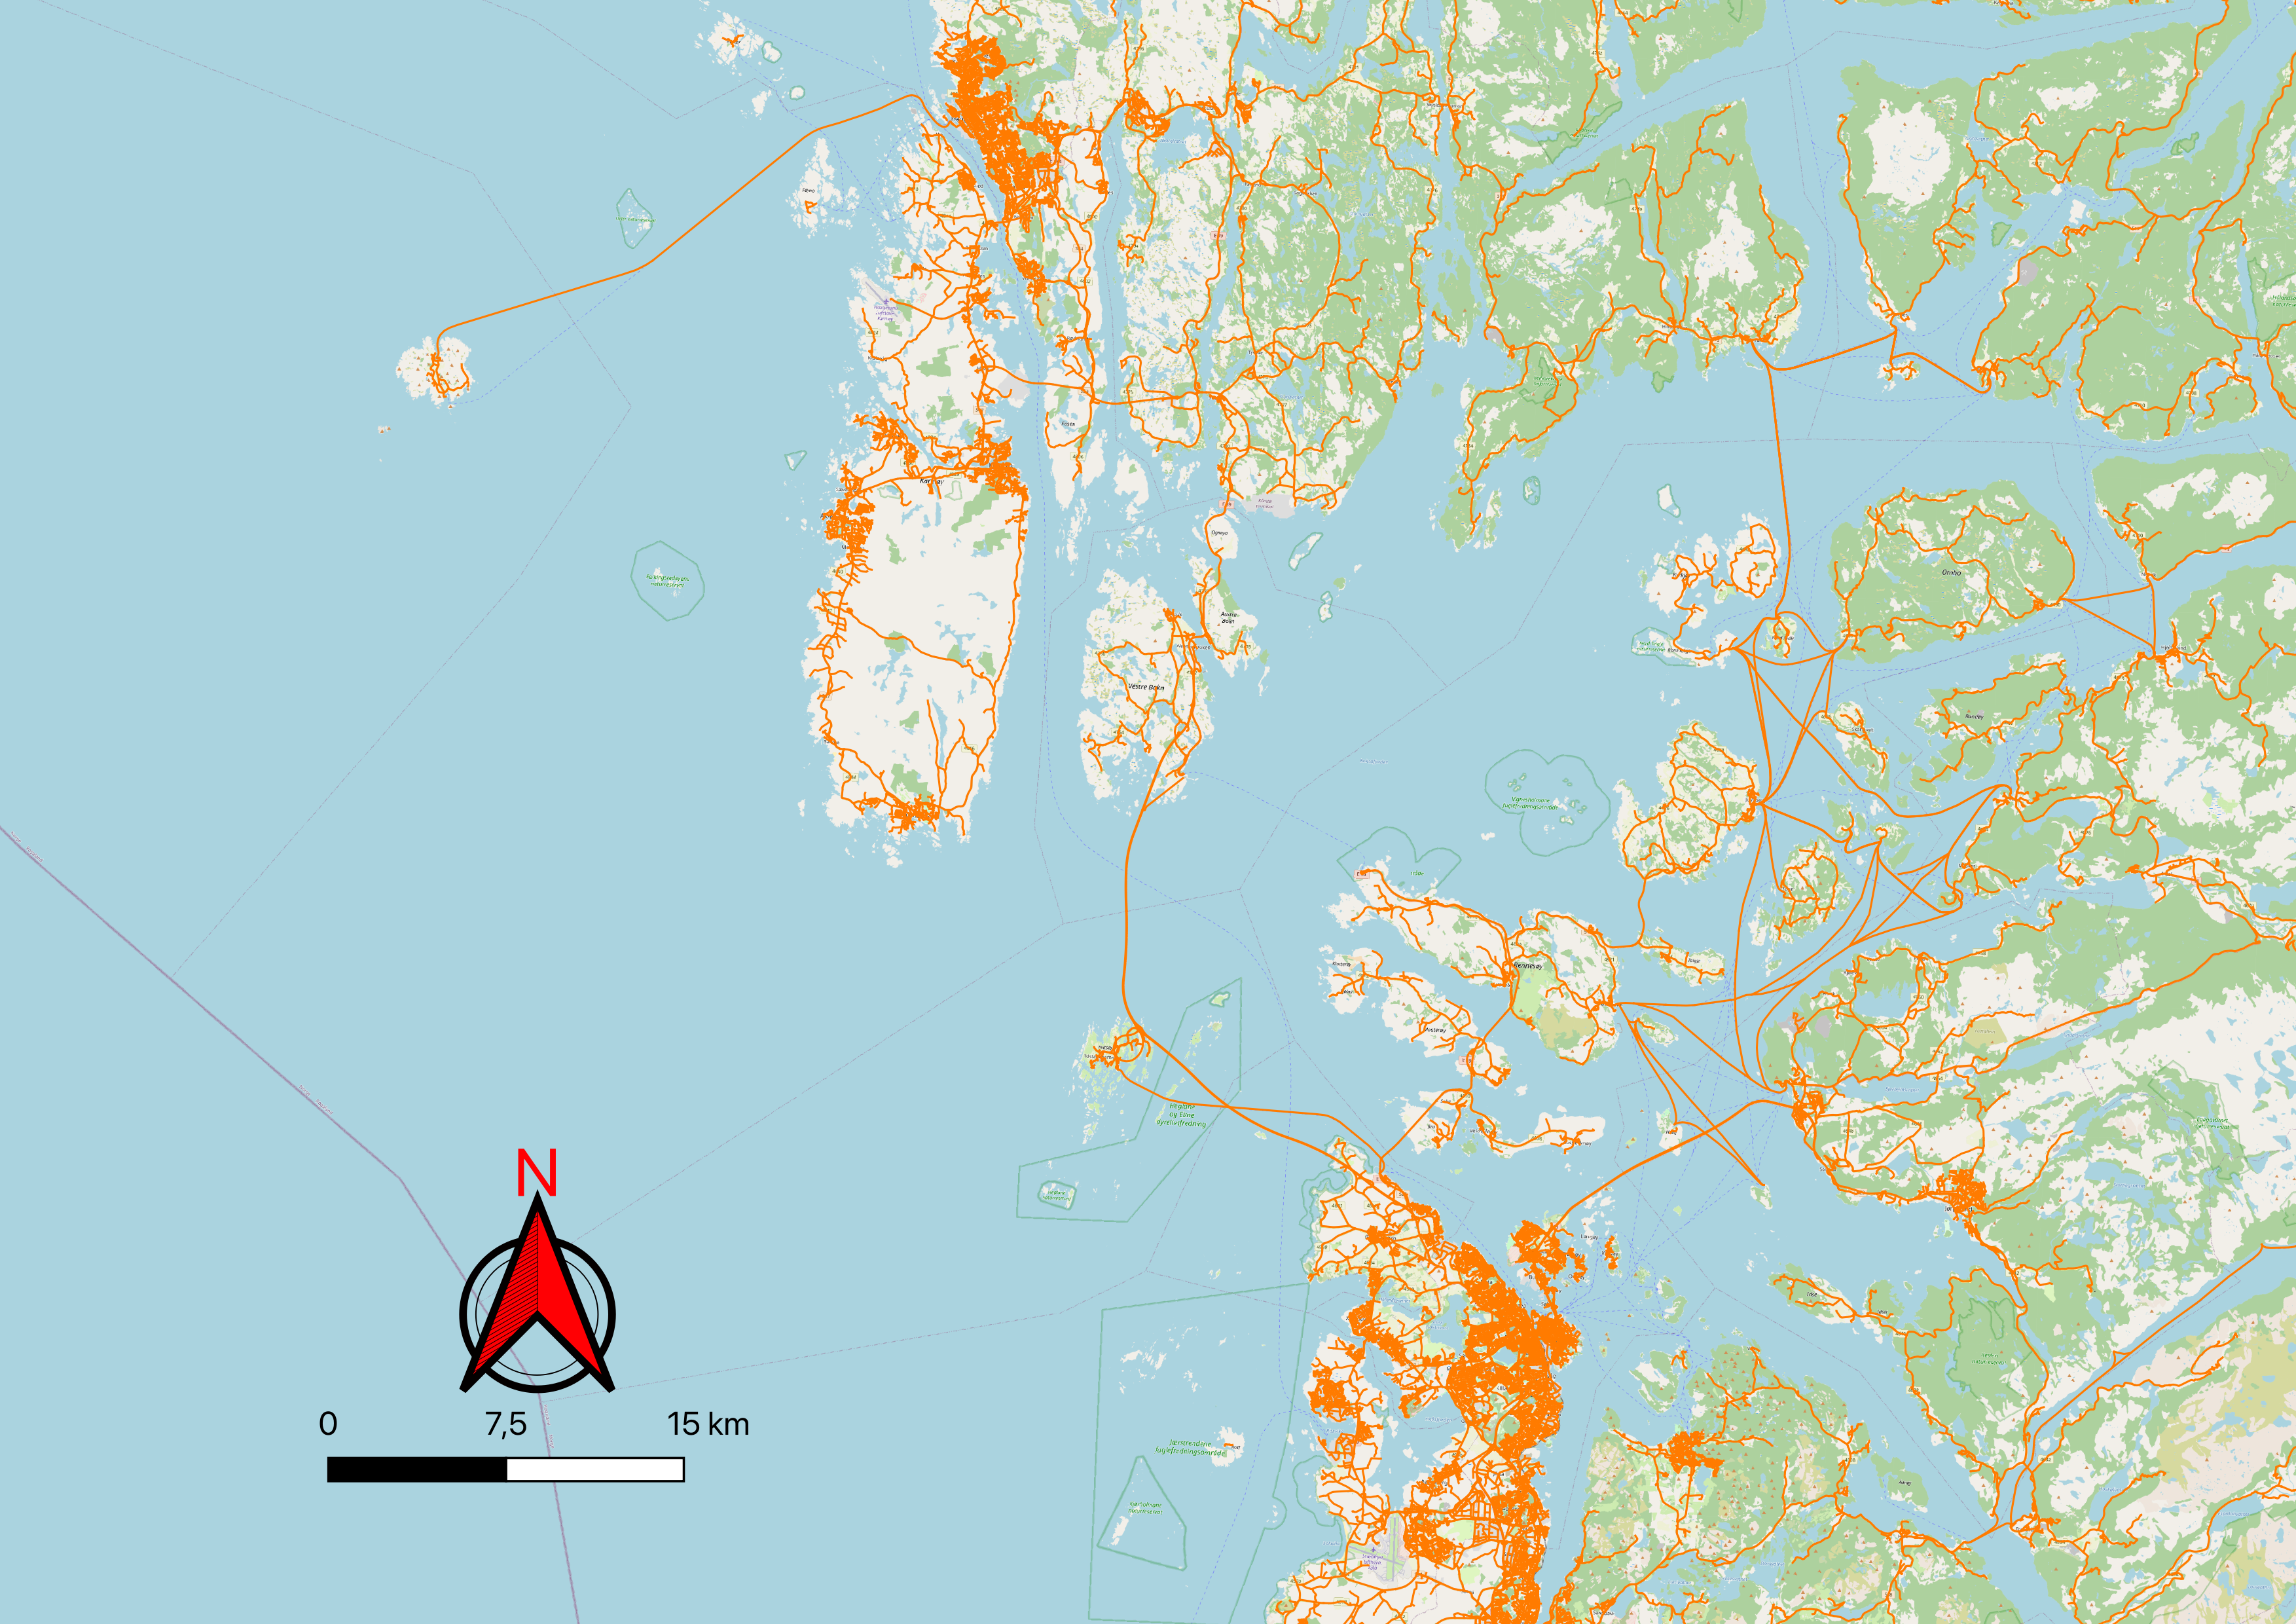
\includegraphics{bilder/Illustrasjon_tunell.png}

}

\caption{\label{fig-prosj-rog}Illustrasjon av vegnett, med Rogfast}

\end{figure}

Ved Rogfast vil man kunne komme helt sør til Bryne og Nærbø på 75
minutter. Reisetid fra Haugaland næringspark ved Rogfast er illustrert i
Figur~\ref{fig-tid-rf} .60 minutters intervallet starter sør i Stavanger
kommune. Reisetiden Gismarvik til Stavanger er estimert til cirka 50
minutter med Rogfast tunnelen. Reisetiden er modellert ut fra vegnettet
i geografien. Mellom alle veiene i ytterpunktene på 75 minutter trekkes
det rette linjer mellom dem. Dette gjør at det fargelagte området som
avsluttes ved 75 minutters intervallet i øst på kartet er illustrert som
en tilnærming med rette linjer.

\begin{figure}[H]

{\centering \includegraphics{bilder/reisetid_rogfast.png}

}

\caption{\label{fig-tid-rf}Avstand fra Gismarvik med Rogfast, målt i
reisetid}

\end{figure}

Tabell~\ref{tbl-rogfast} nedenfor viser summen de som kan gjøre
arbeidsreisen innenfor gitte tidsintervaller, eller kortere. Akkumulerte
tall, som fremstilt i Tabell~\ref{tbl-rogfast}, fanger bedre opp
omfanget av arbeidsmarkedet. Man ser at Rogfasttunnelen øker
rekrutteringsområdet med hele 231\% innenfor 75 minutter. Den største
økningen etter Rogfast er innenfor intervallene 45 og 60 minutter.
Samlet sett øker potensiell sysselsetting i disse intervallene med
759\%. Dette skyldes at store deler av arbeidsmarkedsregionen i
Stavanger blir fanget opp i disse tidsintervallene. Utvidelsen med
Rogfast kommer frem med å sammenligne kartene i Figur~\ref{fig-rtid} og
Figur~\ref{fig-tid-rf}

\hypertarget{tbl-rogfast}{}
\begin{longtable}[]{@{}lll@{}}
\caption{\label{tbl-rogfast}Antall sysselsatte i reisetid fra Haugaland
næringspark som sentrum }\tabularnewline
\toprule()
Reisetid & Uten Rogfast & Med Rogfast \\
\midrule()
\endfirsthead
\toprule()
Reisetid & Uten Rogfast & Med Rogfast \\
\midrule()
\endhead
15 min & 11 273 & 11 273 \\
30 min & 19 310 & 19 466 \\
45 min & 3 045 & 35 896 \\
60 min & 10 586 & 81 128 \\
75 min & 9 784 & 75 164 \\
0-75 min & 53 998 & 178 927 \\
\bottomrule()
\end{longtable}

Med en etablering på Gismarvik vil hovedtyngden av den geografiske
spredningen skje på Haugalandet. Det som er interessant å diskutere er
hvor mye av multiplikatorvirkningene for Haugalandet vil dempes av
rekruttering fra sørsiden av Boknafjorden. Vi vet at arbeidsmarkedet der
sør er større og flere å velge mellom. Det som gjelder her, er
pendlevilligheten til arbeidstakerne. Dette vil variere fra person til
person, men i all hovedsak er det rundt 45 minutter som er bristepunktet
for å pendle eller søke jobb en annen plass. Vi ser i
Figur~\ref{fig-tid-rf} at på 45 minutter kommer vi til Stavanger
sentrum, noe som gjør at Beyonder har gode muligheter til å hente
arbeidskraft sør for Boknafjorden. Vi kan gjøre utregninger på dette med
hjelp av gravitasjonsmodeller, men på grunn av oppgavens
tidsbegrensninger så er det ikke mulig å gjennomføre. Det som kommer
frem, er at noe av multiplikatorvirkningene vil dempes på Haugalandet på
grunn av tilgjengeligheten til Stavanger-regionen. Dette er en av
backwash-effektene som kan oppstå med en slik etablering og
ferdigstilling av Rogfast.

\hypertarget{teori-litteraturgjennomgang}{%
\section{Teori /
Litteraturgjennomgang}\label{teori-litteraturgjennomgang}}

Dette er teori vi har funnet frem og skrevet om, men ikke har noen klar
plass i oppgaven enda:

\hypertarget{klyngeteori}{%
\subsection{Klyngeteori}\label{klyngeteori}}

Klyngeteori er en økonomisk teori som hevder at bedrifter som er
lokalisert i nærheten av hverandre, eller i en klynge, kan ha økonomiske
fordeler som ikke er tilgjengelige for bedrifter som er lokalisert
utenfor klyngen. Denne teorien ble først utviklet av den britiske
økonomen Alfred Marshall i hans bok ``Principles of Economics'' fra
1920.

Marshall (2009) mente at nærhet mellom bedrifter i en klynge kan føre
til økt produktivitet og innovasjon, fordi bedriftene kan dra nytte av
eksternaliteter som kunnskapsoverføring og felles tilgang til
infrastruktur og arbeidskraft. Marshall argumenterte også for at klynger
kan gi bedrifter en økt konkurranseevne ved å tillate dem å dele på
kostnader og risiko.

Senere har forskere videreutviklet Marshalls teori og studert klynger i
ulike sammenhenger. Hoover (1948) undersøkte geografisk lokalisering av
bedrifter og økonomisk aktivitet og argumenterte for at nærhet mellom
bedrifter i en klynge kan føre til reduserte transaksjonskostnader og
økt innovasjon.

Cooke (2001) har også studert klynger og pekt på at klynger kan ha både
positive og negative konsekvenser for økonomisk utvikling. Han
argumenterer for at klynger kan føre til økt innovasjon og
produktivitet, men også til økt økonomisk ulikhet mellom regioner.

Paci og Usai (1999) studerte eksternaliteter og kunnskapsoverføringer i
klynger og fant at kunnskapsspredning mellom bedrifter i en klynge kan
føre til økt innovasjon og produktivitet, spesielt for små og
mellomstore bedrifter. De påpeker imidlertid også at
kunnskapsoverføringen ikke nødvendigvis skjer jevnt mellom alle
bedrifter i klyngen, og at større bedrifter ofte kan dra større nytte av
klyngens ressurser og nettverk.

Henderson (1997) har studert eksternaliteter og industriell utvikling og
funnet at nærhet mellom bedrifter kan føre til økt innovasjon og
produktivitet, men også til økte kostnader på grunn av miljøproblemer og
konkurranse om ressurser.

Glaeser et al. (1992) har studert vekst i byer og funnet at nærhet
mellom bedrifter kan føre til økt innovasjon og produktivitet, men også
til økt konkurranse og konflikt mellom bedrifter.

Samlet sett kan klyngeteori være et nyttig rammeverk for å forstå
økonomisk vekst og utvikling i regioner og byer. Det gir innsikt i
hvordan lokale økonomiske faktorer kan samhandle og skape fordeler og
ulemper for bedrifter i området. Klyngeteorien understreker også
viktigheten av eksterne effekter og kunnskapsspredning, noe som kan
bidra til å stimulere innovasjon og økonomisk vekst i klyngen.

Selv om klyngeteorien har blitt anerkjent som en verdifull tilnærming
til å forstå økonomisk utvikling, har den også møtt kritikk for en rekke
begrensninger og utfordringer. Cooke (2001) argumenterer for at
klyngeteorien kan føre til en overdreven vektlegging av økonomisk
konkurranse innenfor en klynge, og at den ikke tar hensyn til
ikke-markedsmessige faktorer som politikk og kultur. Maskell og Malmberg
(1999) har også pekt på utfordringene med å definere og måle klynger og
deres effekter nøyaktig. Storper (1997) kritiserte klyngeteorien for å
være for lite opptatt av sammenhengen mellom lokale og globale
økonomier. Bathelt et al. (2004) hevder at klyngeteorien overser
viktigheten av kunnskap som flyter gjennom globale nettverk, og at det
er behov for en mer dynamisk og kompleks tilnærming til å forstå
økonomisk utvikling.

Til tross for disse begrensningene, fortsetter klyngeteorien å være et
viktig perspektiv innen økonomisk geografi og regional utvikling.
Forskning innenfor dette feltet vil sannsynligvis fortsette å gi innsikt
i hvordan klynger fungerer, og hvordan de kan bidra til å fremme
økonomisk vekst og utvikling på lokalt og regionalt nivå.

\hypertarget{potensialmuxe5l}{%
\subsection{Potensialmål}\label{potensialmuxe5l}}

Potensialmål innenfor regional økonomi brukes til å estimere det
maksimale nivået av økonomisk aktivitet som en region kan oppnå på lang
sikt, gitt dens tilgjengelige ressurser og teknologi, samt
tilstedeværelsen av næringsklynger. Den faktiske produksjonen er den
mengden varer og tjenester som faktisk produseres i en region, mens den
potensielle produksjonskapasiteten er den mengden av varer og tjenester
som kan produseres med eksisterende ressurser og teknologi (Fujita et
al., 1999). Potensialmål brukes ofte til å evaluere økonomisk ytelse og
muligheter for økonomisk vekst i en region. Likevel, et nøyaktig estimat
av potensialmålet er veldig krevende, da det er avhengig av en rekke
faktorer som kan endre seg over tid (Fujita et al., 1999).

\newpage

\hypertarget{references}{%
\subsection*{References}\label{references}}
\addcontentsline{toc}{subsection}{References}

\hypertarget{refs}{}
\begin{CSLReferences}{1}{0}
\leavevmode\vadjust pre{\hypertarget{ref-akersolutions2021}{}}%
Aker Solutions. (2021, oktober 14). \emph{Aker {Solutions}, {DeepOcean}
and {Solstad Offshore Create Offshore Renewables Alliance}}. {Aker
Solutions}.
\url{https://akersolutions.com/news/news-archive/2021/aker-solutions-deepocean-and-solstad-offshore-create-offshore-renewables-alliance/}

\leavevmode\vadjust pre{\hypertarget{ref-alonso1964a}{}}%
Alonso, W. (1964). \emph{Location and {Land Use}: {Toward} a {General
Theory} of {Land Rent}}. {Harvard University Press}.

\leavevmode\vadjust pre{\hypertarget{ref-andrews1953}{}}%
Andrews, R. B. (1953). Mechanics of the {Urban Economic Base}:
{Historical Development} of the {Base Concept}. \emph{Land Economics},
\emph{29}(2), 161--167. \url{https://doi.org/10.2307/3144408}

\leavevmode\vadjust pre{\hypertarget{ref-andrews1954}{}}%
Andrews, R. B. (1954). Mechanics of the {Urban Economic Base}: {The
Problem} of {Base Measurement}. \emph{Land Economics}, \emph{30}(1),
52--60. \url{https://doi.org/10.2307/3144917}

\leavevmode\vadjust pre{\hypertarget{ref-audretsch1996}{}}%
Audretsch, D. B., og Feldman, M. P. (1996). R\&{D Spillovers} and the
{Geography} of {Innovation} and {Production}. \emph{The American
Economic Review}, \emph{86}(3), 630--640.
\url{https://www.jstor.org/stable/2118216}

\leavevmode\vadjust pre{\hypertarget{ref-bathelt2004}{}}%
Bathelt, H., Malmberg, A., og Maskell, P. (2004). \emph{Clusters and
Knowledge: Local Buzz, Global Pipelines and the Process of Knowledge
Creation}. \url{https://doi.org/10.1191/0309132504ph469oa}

\leavevmode\vadjust pre{\hypertarget{ref-bayer2015}{}}%
Bayer, S. B., Harstad, M., og Gressgård, Leif Jarle. (2015).
\emph{Regionale effekter som følge av Rogfast og Ryfast}.
\url{https://norceresearch.brage.unit.no/norceresearch-xmlui/bitstream/handle/11250/2631626/Rapport\%20IRIS\%202015-092\%20Regionforst\%c3\%b8rring\%20Infrastrukturprosjekter.pdf?sequence=1\&isAllowed=y}

\leavevmode\vadjust pre{\hypertarget{ref-beyonder2023}{}}%
Beyonder. (2023a). \emph{Beyonder}. {Beyonder}.
\url{https://www.beyonder.no}

\leavevmode\vadjust pre{\hypertarget{ref-beyonder2023a}{}}%
Beyonder. (2023b). \emph{Technology}. {Beyonder}.
\url{https://www.beyonder.no/technology}

\leavevmode\vadjust pre{\hypertarget{ref-boudeville1964}{}}%
Boudeville, J. R. (1964). Les Pôles de Croissance En Question.
\emph{Revue économique}, \emph{15}(1), 75--104.

\leavevmode\vadjust pre{\hypertarget{ref-capello2015}{}}%
Capello, R. (2015). \emph{Regional {Economics}}. {Routledge}.
\url{https://doi.org/10.4324/9781315720074}

\leavevmode\vadjust pre{\hypertarget{ref-cooke2001}{}}%
Cooke, P. (2001). Regional {Innovation Systems}, {Clusters}, and the
{Knowledge Economy}. \emph{Industrial and Corporate Change},
\emph{10}(4), 945--974. \url{https://doi.org/10.1093/icc/10.4.945}

\leavevmode\vadjust pre{\hypertarget{ref-cowi2012}{}}%
Cowi. (2012). \emph{E39 ROGFAST - REGULERINGSPLANER PLANBESKRIVELSE}.
\url{https://www.vegvesen.no/globalassets/vegprosjekter/utbygging/e39rogfast/vedlegg/reguleringsplanar/e39-rogfast-planbeskrivelse.pdf}

\leavevmode\vadjust pre{\hypertarget{ref-duranton2000}{}}%
Duranton, G., og Puga, D. (2000). Diversity and {Specialisation} in
{Cities}: {Why}, {Where} and {When Does} It {Matter}? \emph{Urban
Studies}, \emph{37}(3), 533--555.
\url{https://doi.org/10.1080/0042098002104}

\leavevmode\vadjust pre{\hypertarget{ref-duranton2003}{}}%
Duranton, G., og Puga, D. (2003). \emph{Micro-{Foundations} of {Urban
Agglomeration Economies}} (Nr. w9931; s. w9931). {National Bureau of
Economic Research}. \url{https://doi.org/10.3386/w9931}

\leavevmode\vadjust pre{\hypertarget{ref-duranton2004}{}}%
Duranton, G., og Puga, D. (2004). Chapter 48 - {Micro-Foundations} of
{Urban Agglomeration Economies}. I J. V. Henderson og J.-F. Thisse
(Red.), \emph{Handbook of {Regional} and {Urban Economics}} (Bd. 4, s.
2063--2117). {Elsevier}.
\url{https://doi.org/10.1016/S1574-0080(04)80005-1}

\leavevmode\vadjust pre{\hypertarget{ref-ferde2023a}{}}%
Ferde. (2023a). \emph{Haugalandspakken - Hva betaler du i bompenger?}
{Ferde.no}. \url{https://ferde.no/bomanlegg-og-priser/haugalandspakken}

\leavevmode\vadjust pre{\hypertarget{ref-ferde2023}{}}%
Ferde. (2023b). \emph{T-forbindelsen}. {Ferde.no}.
\url{https://ferde.no/bomanlegg-og-priser/t-forbindelsen}

\leavevmode\vadjust pre{\hypertarget{ref-fornybarnorge2022}{}}%
FornybarNorge. (2022, desember 6). \emph{Havvind}.
\url{https://www.fornybarnorge.no/havvind/}

\leavevmode\vadjust pre{\hypertarget{ref-fujita1999}{}}%
Fujita, M., Krugman, P., og Venables, A. J. (1999). \emph{The {Spatial
Economy}: {Cities}, {Regions}, and {International Trade}}.
\url{https://doi.org/10.7551/mitpress/6389.001.0001}

\leavevmode\vadjust pre{\hypertarget{ref-glaeser2010}{}}%
Glaeser, E. L. (Red.). (2010). \emph{Agglomeration {Economics}}.
{University of Chicago Press}.
\url{https://press.uchicago.edu/ucp/books/book/chicago/A/bo8143498.html}

\leavevmode\vadjust pre{\hypertarget{ref-glaeser1992}{}}%
Glaeser, E. L., Kallal, H. D., Scheinkman, J. A., og Shleifer, A.
(1992). Growth in {Cities}. \emph{Journal of Political Economy},
\emph{100}(6), 1126--1152. \url{https://doi.org/10.1086/261856}

\leavevmode\vadjust pre{\hypertarget{ref-ha2012}{}}%
Ha, S. J., og Swales, J. K. (2012). The Export-Base Model with a
Supply-Side Stimulus to the Export Sector. \emph{The Annals of Regional
Science}, \emph{49}(2), 323--353.
\url{https://doi.org/10.1007/s00168-010-0423-3}

\leavevmode\vadjust pre{\hypertarget{ref-haugalandnaeringspark2023a}{}}%
Haugaland næringspark. (2023, februar 10). \emph{Parken}. {Haugaland
Næringspark}. \url{https://haugaland-park.no/parken/}

\leavevmode\vadjust pre{\hypertarget{ref-henderson1997}{}}%
Henderson, V. (1997). Externalities and {Industrial Development}.
\emph{Journal of Urban Economics}, \emph{42}(3), 449--470.
\url{https://doi.org/10.1006/juec.1997.2036}

\leavevmode\vadjust pre{\hypertarget{ref-hirschman1958}{}}%
Hirschman, A. O. (1958). \emph{The {Strategy} of {Economic
Development}}. {Yale University Press}.

\leavevmode\vadjust pre{\hypertarget{ref-hoover1948}{}}%
Hoover, E. M. (1948). \emph{The Location of Economic Activity}.
{McGraw-Hill Book Company}.

\leavevmode\vadjust pre{\hypertarget{ref-hoyt1954}{}}%
Hoyt, H. (1954). Homer {Hoyt} on {Development} of {Economic Base
Concept}. \emph{Land Economics}, \emph{30}(2), 182--186.
\url{https://doi.org/10.2307/3144940}

\leavevmode\vadjust pre{\hypertarget{ref-isserman2007}{}}%
Isserman, A. M. (2007). \emph{The {Location Quotient Approach} to
{Estimating Regional Economic Impacts}}.
\url{https://doi.org/10.1080/01944367708977758}

\leavevmode\vadjust pre{\hypertarget{ref-kristensen2022}{}}%
Kristensen, S. (2022, juni 8). \emph{Er det planlagt et nytt luftslott
på Gismarvik?} {Haugesunds Avis}.
\url{https://www.h-avis.no/5-62-1356620}

\leavevmode\vadjust pre{\hypertarget{ref-krugman1991}{}}%
Krugman, P. (1991). Increasing {Returns} and {Economic Geography}.
\emph{The Journal of Political Economy}, \emph{99}(3), 483--499.
\url{https://doi.org/10.1086/261763}

\leavevmode\vadjust pre{\hypertarget{ref-leigh1970}{}}%
Leigh, R. (1970). The {Use} of {Location Quotients} in {Urban Economic
Base Studies}. \emph{Land Economics}, \emph{46}(2), 202--205.
\url{https://doi.org/10.2307/3145181}

\leavevmode\vadjust pre{\hypertarget{ref-leontief1986}{}}%
Leontief, W. (1986). \emph{Input-{Output Economics}}. {Oxford University
Press}. \url{https://books.google.com?id=HMnQCwAAQBAJ}

\leavevmode\vadjust pre{\hypertarget{ref-marshall2009}{}}%
Marshall, A. (2009). \emph{Principles of {Economics}: {Unabridged Eighth
Edition}}. {Cosimo, Inc.}

\leavevmode\vadjust pre{\hypertarget{ref-maskell1999}{}}%
Maskell, P., og Malmberg, A. (1999). Localised Learning and Industrial
Competitiveness. \emph{Cambridge Journal of Economics}, \emph{23}(2),
167--185. \url{https://doi.org/10.1093/cje/23.2.167}

\leavevmode\vadjust pre{\hypertarget{ref-mattila1955}{}}%
Mattila, J. M., og Thompson, W. R. (1955). The {Measurement} of the
{Economic Base} of the {Metropolitan Area}. \emph{Land Economics},
\emph{31}(3), 215--228. \url{https://doi.org/10.2307/3159415}

\leavevmode\vadjust pre{\hypertarget{ref-mccann2013}{}}%
McCann, P. (2013). \emph{Modern Urban and Regional Economics} (2nd ed.).
{University Press}.

\leavevmode\vadjust pre{\hypertarget{ref-miller2009}{}}%
Miller, R. E., og Blair, P. D. (2009). \emph{Input-{Output Analysis}:
{Foundations} and {Extensions}}. {Cambridge University Press}.
\url{https://books.google.com?id=viHaAgAAQBAJ}

\leavevmode\vadjust pre{\hypertarget{ref-ntb2008}{}}%
NTB. (2008, november 26). \emph{Hydro stenger Søderberg-anlegget}.
\url{https://www.bt.no/nyheter/okonomi/i/XoJnW/hydro-stenger-soederberg-anlegget}

\leavevmode\vadjust pre{\hypertarget{ref-ntb2016}{}}%
Ntb. (2016, mai 18). \emph{Oljekrisen har ført til 25.000 færre
arbeidsplasser}.
\url{https://www.aftenposten.no/okonomi/i/vQwgw/oljekrisen-har-foert-til-25000-faerre-arbeidsplasser}

\leavevmode\vadjust pre{\hypertarget{ref-haugalandnaeringspark2023}{}}%
næringspark, H. (2023). \emph{Havnen}. {Haugaland Næringspark}.
\url{https://haugaland-park.no/havnen/}

\leavevmode\vadjust pre{\hypertarget{ref-paci1999}{}}%
Paci, R., og Usai, S. (1999). Externalities, Knowledge Spillovers and
the Spatial Distribution of Innovation. \emph{GeoJournal}, \emph{49}(4),
381--390. \url{https://doi.org/10.1023/A:1007192313098}

\leavevmode\vadjust pre{\hypertarget{ref-perroux1955}{}}%
Perroux, F. (1955). Note Sur La Notion de Póle de Croissance.
\emph{Economie Appliquee}, \emph{8}(2), 307--320.
\url{https://www.semanticscholar.org/paper/Note-sur-la-notion-de-p\%C3\%B3le-de-croissance-Perroux-Perroux/997ddab3289d6aee27390b5e95914b3bd4c60a8e}

\leavevmode\vadjust pre{\hypertarget{ref-pfouts1958}{}}%
Pfouts, R. W., og Curtis, E. T. (1958). Limitations of the {Economic
Base Analysis}. \emph{Social Forces}, \emph{36}(4), 303--310.
\url{https://doi.org/10.2307/2573967}

\leavevmode\vadjust pre{\hypertarget{ref-proff2023}{}}%
Proff. (2023). \emph{Thomas {Søyland Hagen} - 917015961 - {Sandnes} -
{Se Regnskap}, {Roller} Og Mer}.
\url{https://www.proff.no/selskap/thomas-s\%C3\%B8yland-hagen/sandnes/batterier/IF5YU1L000E/}

\leavevmode\vadjust pre{\hypertarget{ref-sjofartsdirektoratet2023}{}}%
Sjøfartsdirektoratet. (2023, februar 22). \emph{Sjøfartsdirektoratets
historie}.
\url{https://www.sdir.no/om-direktoratet/presentasjon-av-direktoratet/sjofartsdirektoratets-historie/}

\leavevmode\vadjust pre{\hypertarget{ref-ssb2023}{}}%
SSB. (2023). \emph{Standard for Næringsgruppering ({SN})}.
\url{https://www.ssb.no/klass/klassifikasjoner/6}

\leavevmode\vadjust pre{\hypertarget{ref-stabler1968}{}}%
Stabler, J. C. (1968). Exports and {Evolution}: {The Process} of
{Regional Change}. \emph{Land Economics}, \emph{44}(1), 11--23.
\url{https://doi.org/10.2307/3159606}

\leavevmode\vadjust pre{\hypertarget{ref-statensvegvesen}{}}%
Statens vegvesen. (u.å.). \emph{Vegkart}. {Statens vegvesen}. Hentet 2.
mai 2023, fra
\url{https://www.vegvesen.no/fag/teknologi/nasjonal-vegdatabank/hente-ut-og-se-pa-data-i-nasjonal-vegdatabank/kart/}

\leavevmode\vadjust pre{\hypertarget{ref-statensvegvesen2023}{}}%
Statens vegvesen. (2023, januar 9). \emph{E39 Rogfast}. {Statens
vegvesen}.
\url{https://www.vegvesen.no/vegprosjekter/europaveg/e39rogfast/}

\leavevmode\vadjust pre{\hypertarget{ref-stokka2014}{}}%
Stokka, O. K. (2014, mars 8). \emph{Nå skal gatekampen avgjøres}.
\url{https://www.aftenbladet.no/lokalt/i/vwz1L/naa-skal-gatekampen-avgjoeres}

\leavevmode\vadjust pre{\hypertarget{ref-storper1997}{}}%
Storper, M. (1997). \emph{The {Regional World}: {Territorial
Development} in a {Global Economy}}. {Guilford Press}.
\url{https://books.google.com?id=ROaCVd6RRN8C}

\leavevmode\vadjust pre{\hypertarget{ref-storksen2022a}{}}%
Størksen, T. (2022a, juli 28). \emph{(+) Usikkerhet om fortsatt drift
for Beyonder}. {Haugesunds Avis}.
\url{https://www.h-avis.no/5-62-1387766}

\leavevmode\vadjust pre{\hypertarget{ref-storksen2022}{}}%
Størksen, T. (2022b, september 14). \emph{(+) Beyonder: -- Tar tid å
hente milliarder}. {Haugesunds Avis}.
\url{https://www.h-avis.no/5-62-1409673}

\leavevmode\vadjust pre{\hypertarget{ref-storksen2023}{}}%
Størksen, T. (2023, januar 29). \emph{(+) Beyonder leter fremdeles etter
penger}. {Haugesunds Avis}. \url{https://www.h-avis.no/5-62-1476940}

\leavevmode\vadjust pre{\hypertarget{ref-thomas1964}{}}%
Thomas, M. D. (1964). The {Export Base} and {Development Stages
Theories} of {Regional Economic Growth}: {An Appraisal}. \emph{Land
Economics}, \emph{40}(4), 421--432.
\url{https://doi.org/10.2307/3144479}

\leavevmode\vadjust pre{\hypertarget{ref-thorsnaes2021}{}}%
Thorsnæs, G. (2021). Haugalandet. I \emph{Store norske leksikon}.
\url{https://snl.no/Haugalandet}

\leavevmode\vadjust pre{\hypertarget{ref-whiteaker2022}{}}%
Whiteaker, J. (2022, april 13). \emph{What Is a Gigafactory and Where
Are They Being Built?} {Investment Monitor}.
\url{https://www.investmentmonitor.ai/manufacturing/what-is-a-gigafactory-where-are-they-being-built}

\end{CSLReferences}



\end{document}
